\chapter{Background}
\addcontentsline{toc}{chapter}{Background}
\chaptermark{Background}
\label{sec:background}
A fundamental understanding of the data produced by the sequencing of biological organisms is essential for comprehending the research outlined in this manuscript. If you are already familiar with DNA sequences, how they are obtained, and how they differ between species or individuals, you may proceed to Section~\ref{sec:background_pangenomics} \emph{From reads to \kmers}.
\section{DNA, genome variation and sequencing data}
\label{sec:dna}
\gls{DNA} (Deoxyribonucleic Acid) is a complex molecule with a double helix structure that carries the genetic information of an organism. Although its discovery was the result of the cumulative work of many scientists over nearly 90 years, the currently accepted model was first correctly described through the work of James Watson and Francis Crick, along with Maurice Wilkins and Rosalind Franklin, between 1951 and 1953 in Cambridge, UK~\cite{franklin}.\\
The information encoded in DNA provides the instructions for an organism to develop, survive in its environment, and reproduce. These instructions are stored as a sequence of monomers called nucleotides. Each nucleotide consists of a sugar, a phosphate group, and one of four nucleobases: cytosine, guanine, adenine, and thymine. Nucleotides are typically represented by the first letter of their respective nucleobase: A, C, G, and T. In \gls{RNA} (a different molecule that acts as transcription of DNA), thymine is replaced by uracil.\\
The nucleotides are linked by a sugar-phosphate backbone, and hydrogen bonds between complementary nucleotides stabilize the molecule's double-stranded structure: A pairs with T, and C pairs with G. This pairing is crucial for both DNA replication and protein synthesis. Figure~\ref{fig:DNA} illustrates the structure of the DNA molecule and its nucleotides, as initially drawn by Francis Crick in 1953.
\begin{figure}[!ht]
	\centering
	\begin{subfigure}[b]{0.95\textwidth}
		\centering
		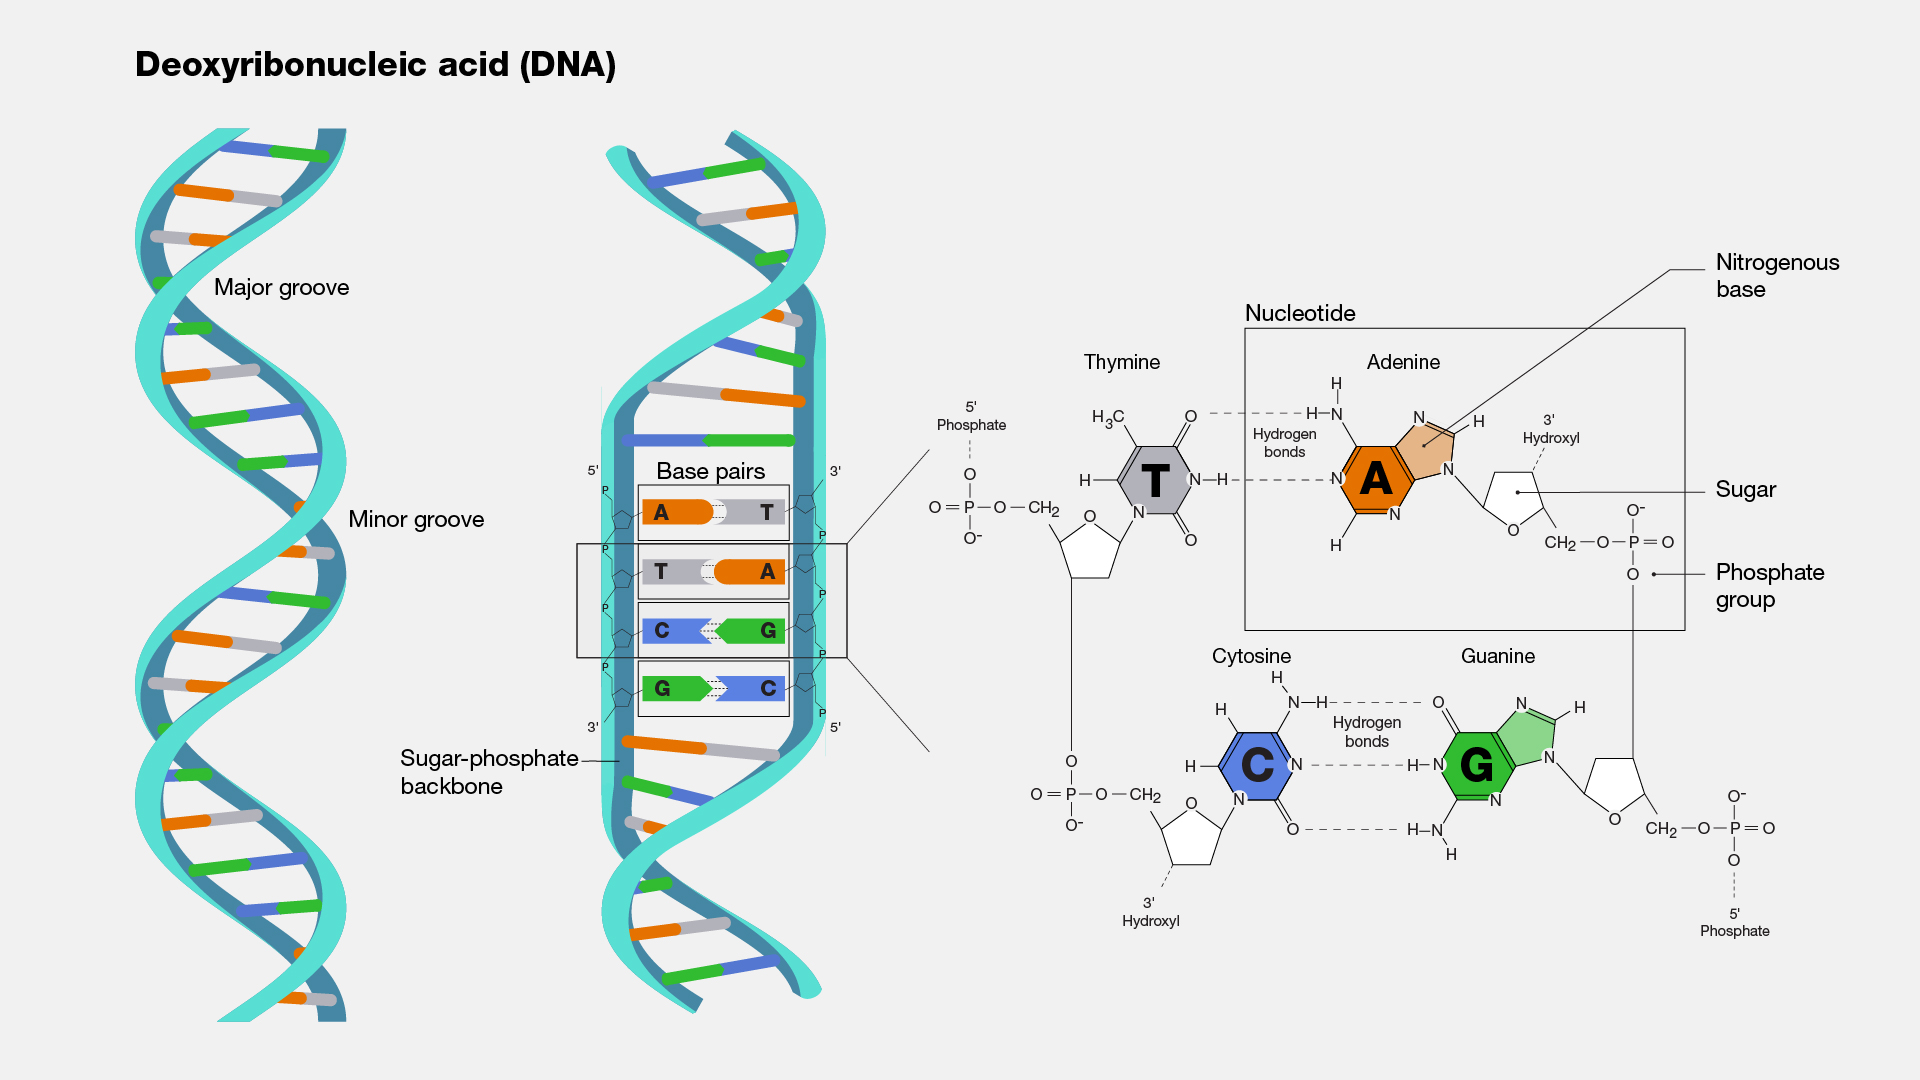
\includegraphics[width=0.95\textwidth]{figures/background/DNA_2024a.jpg}
		\caption[The DNA molecule]{The DNA molecule and the structure of the nucleotides, the basic piece of information of the DNA. Figure from \gls{NIH} glossary~\cite{nih_dna}.} 
	\end{subfigure}%
	\\
	\begin{subfigure}[b]{0.75\textwidth}
		\centering
		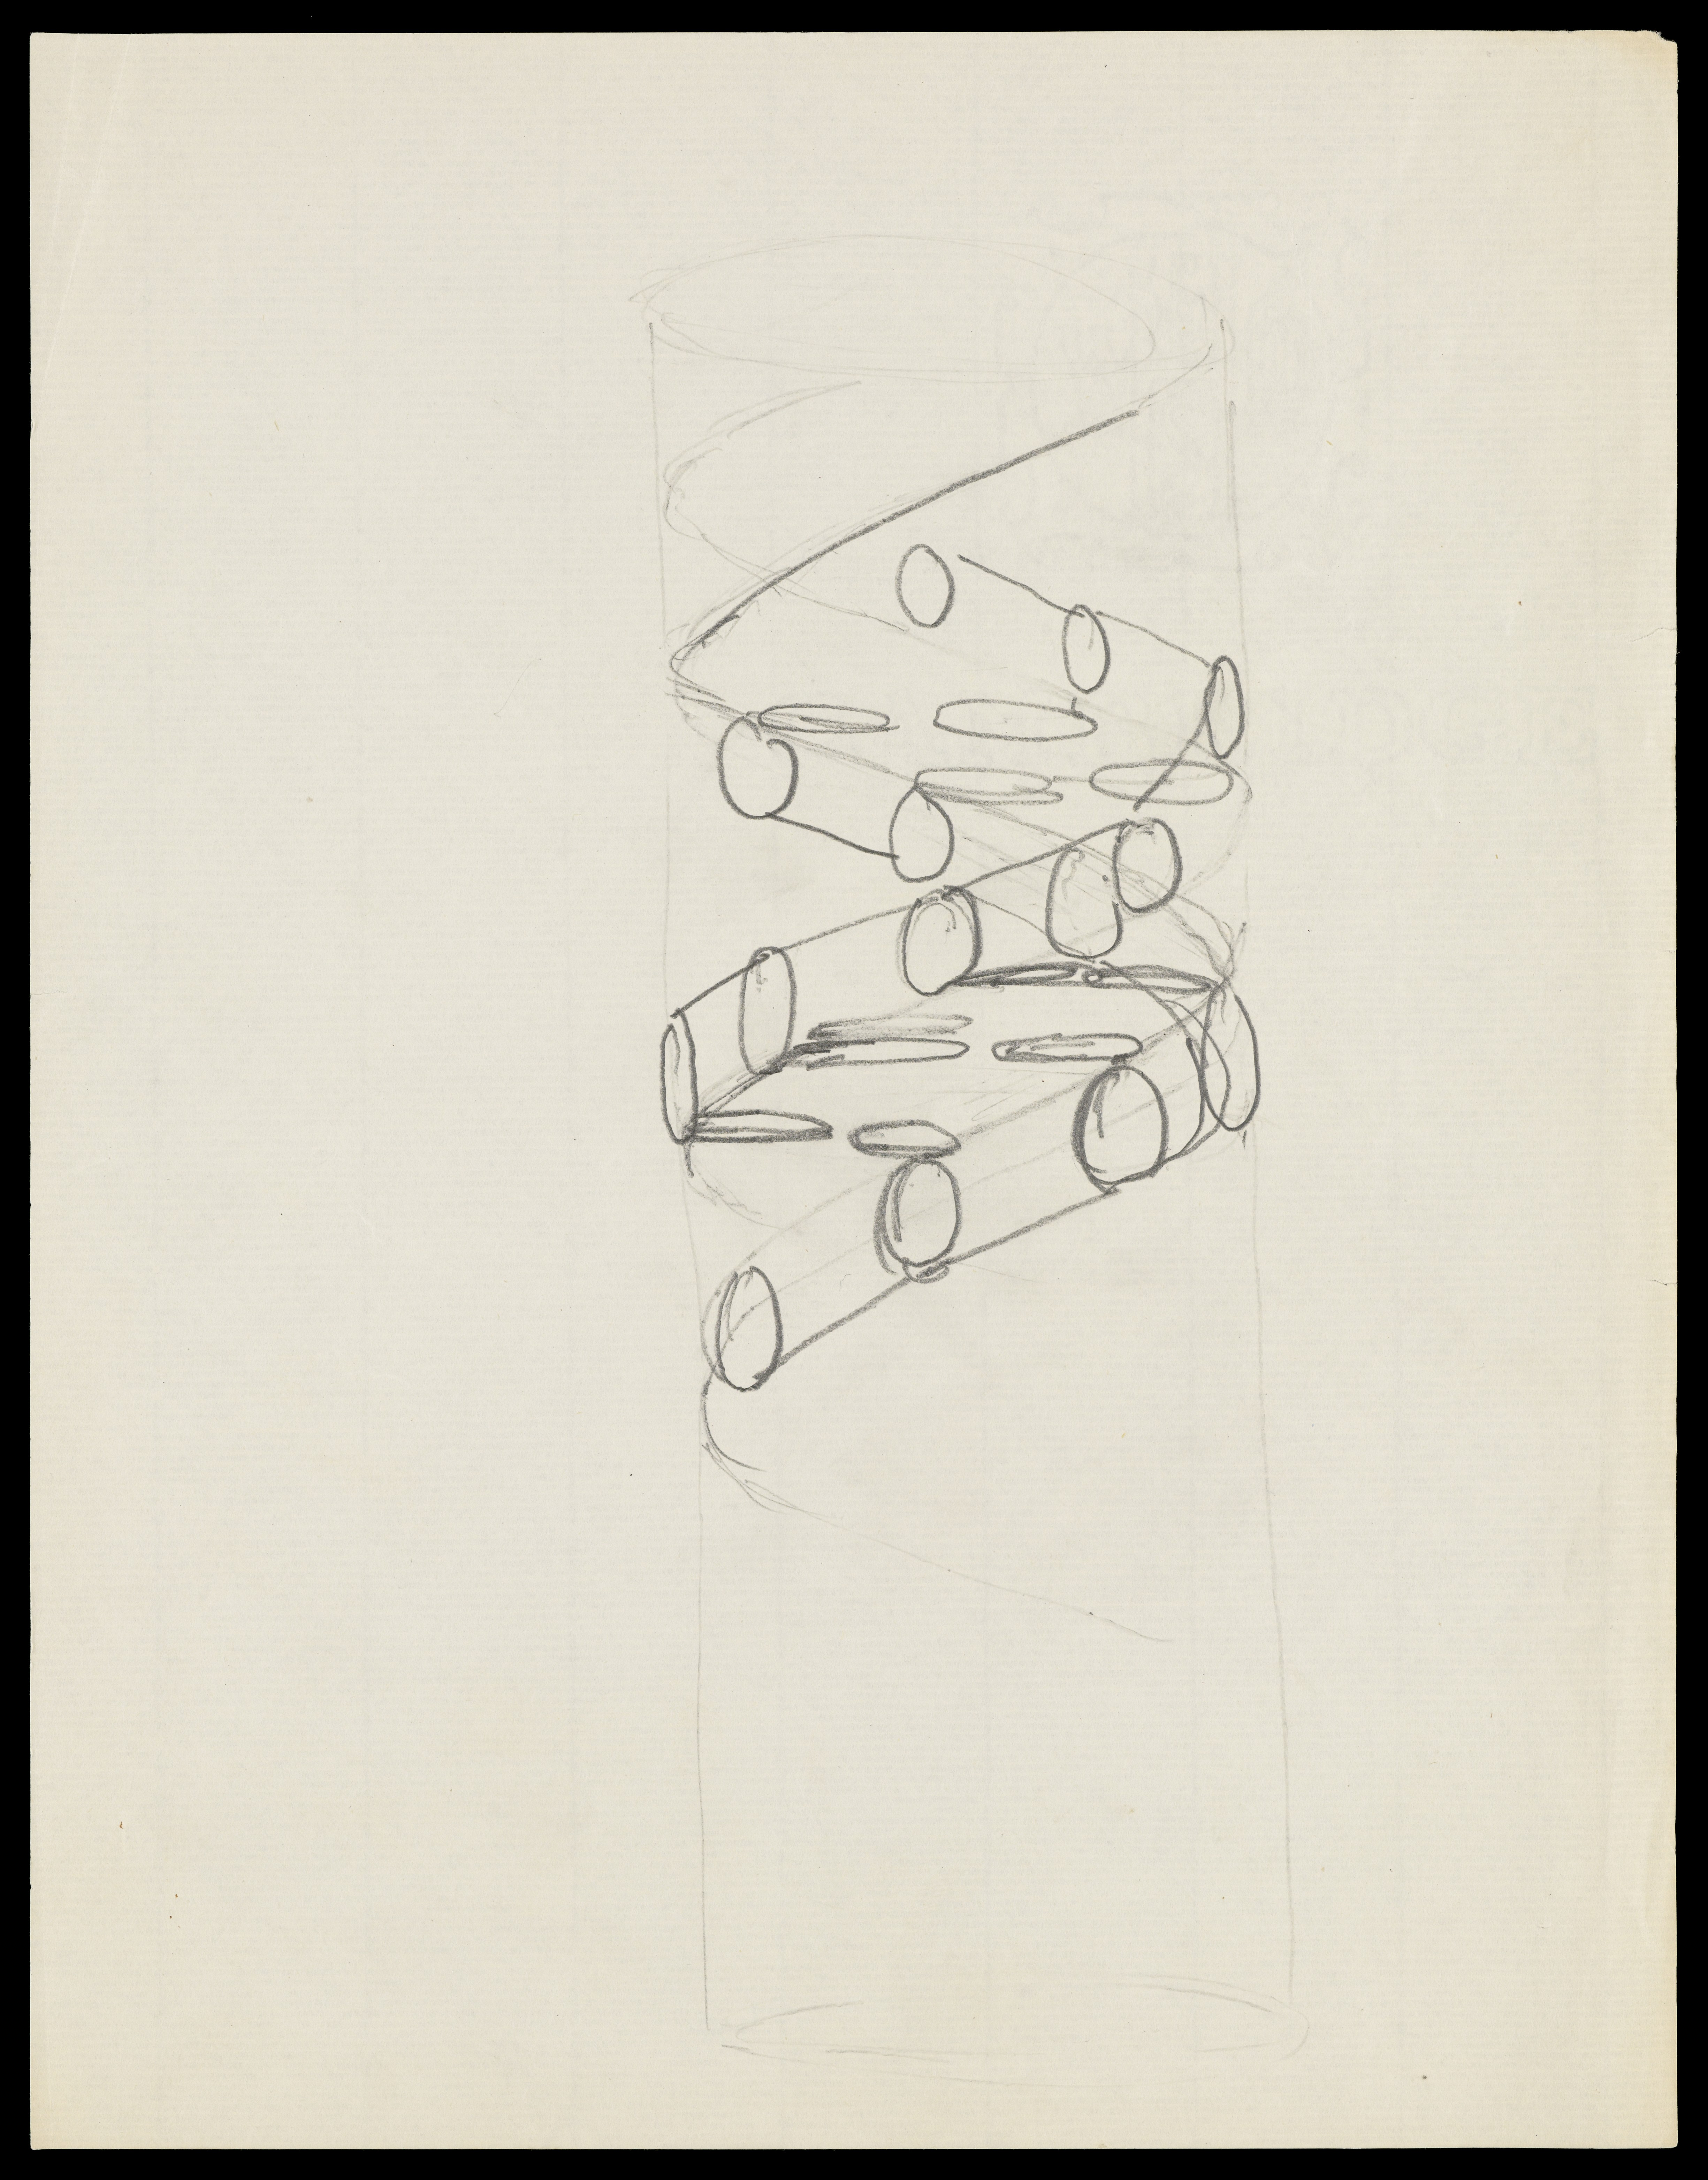
\includegraphics[width=0.5\textwidth]{figures/background/DNA_sketch.jpg}
		\caption[The DNA sketch by Crick]{The DNA molecule model draw by Francis Crick in 1953.} 
	\end{subfigure}%
\caption{The DNA molecule.}
\label{fig:DNA}
\end{figure}

To fit within the cell nucleus, DNA is organized into highly compact structures. First, it is coiled around proteins called histones, forming a compact structure known as chromatin. The chromatin further forms loops, which are held in place by other molecules to create the structure of a chromosome. Chromosomes are inherited by offspring through sexual or asexual reproduction. Humans are diploid organisms—meaning they contain two copies of each chromosome—one inherited from the mother (via the egg) and one from the father (via the sperm). Both the egg and the sperm (collectively called gametes) contain one copy of each chromosome. While mammals are typically diploid, other organisms can be haploid (containing a single copy of each chromosome) or polyploid, meaning they possess more than two copies of each chromosome. For example, sugarcane, the world's most harvested crop by tonnage, can have more than eight copies of a chromosome, reaching up to twelve~\cite{sugarcane}.
The complete set of genetic material present in a cell is the genome. In humans, each nucleus of non-reproductive cells contains 23 pairs of chromosomes. Of these, 22 pairs are autosomes, which are chromosomes that are not involved in determining sex and are common to both sexes. The 23rd pair is the sex chromosomes, which consist of either two copies of the X chromosome for females or one X and one Y chromosome for males. The telomere forms the end part of the chromosome, while the centromere is located in the central region. Telomeres protect chromosome ends by blocking DNA damage repair mechanisms. In humans, telomeres are composed of consecutive repeats of the sequence \texttt{TTAGGG} s, which span 5 to 15 thousand bases. As the ends of chromosomes cannot be fully replicated during cell division, telomeres naturally shorten with each division, contributing to the aging process, though the repeated sequence itself does not change. Abnormal telomere length can lead to genetic defects and diseases~\cite{telomeres}. In contrast to the relatively stable structure of the telomere, the centromere is one of the most rapidly mutating regions of the human genome. Its sequence is organized into Higher Order Repeats (\gls{HOR}), which consist of consecutive copies of large sections containing multiple repetitions of smaller sub-sequences. Centromeres are the most challenging regions to reconstruct from sequencing data~\cite{centromeres}.
%Both of these regions are known to contain large amounts of repetitive sequences, which are particularly challenging to reconstruct accurately from sequencing data.

Finally, there is also the mitochondrial genome, which is located outside the nucleus. It has a circular structure and is primarily maternally inherited.

\subsection{DNA sequencing}
In many biological disciplines, studying an organism's genetic information contained in its DNA is essential. Over the years, researchers have developed various methods and techniques to sequentially read nucleotides from cellular DNA; these techniques are collectively referred to as genome sequencing. The result of these processes is a collection of sequence reads, often simply called "reads," which represent the nucleotide sequences observed in the input DNA molecules. By sequencing DNA fragments and computationally assembling them, we can observe genomes~\cite{garrison_pangenome}. Genome assembly is a computational process used to reconstruct the complete genome sequence of an organism from a set of reads generated by one or more sequencing techniques.\\
Sequencing typically involves three main steps. Below, I describe them with significant simplifications to provide a brief overview:
\begin{itemize}[leftmargin=1.8cm]
	\item[\textbf{Library preparation}] The first step requires several hours of nontrivial biological manipulation of samples to extract and purify DNA from the cell nucleus without causing damage. This process isolates the genetic material from other cellular components, such as RNA and proteins. The DNA molecules are then fragmented into pieces of varying lengths, followed by ligation of $5\prime$ and $3\prime$ adapters. Some technologies require \gls{PCR} amplification of fragments, while others do not.
	\item[\textbf{Sequencing}]Next, specialized machines detect the sequence of nucleotides that make up the extracted DNA fragments. These processes, referred to as sequencing, employ various—often proprietary—technologies to determine the precise order of nucleotides (A, C, G, and T) in a DNA molecule. The raw data generated by these machines consist of sequences of characters, commonly referred to as sequencing reads or simply reads.
	\item[\textbf{Analysis}] In this step, quality control (\gls{QC}) is usually performed to remove adapters and reads that are too short or of low quality. Typically, the first step after QC is either the assembly of the sequences or their input into a workflow specific to the intended application.
\end{itemize}
The landscape of DNA sequencing has evolved significantly since its inception. In 1977, Frederick Sanger and his colleagues introduced the first widely adopted sequencing method, known as chain termination sequencing, or Sanger sequencing~\cite{sanger_sequencing}. This technique enabled the reliable and reproducible determination of nucleotide sequences in a DNA molecule for the first time. It was the method used to achieve the first sequencing of mitochondrial DNA and the first (almost) complete human genome in 2001 ~\cite{mitochondrialDNA,first_human_genome}. Sanger sequencing, through gel-based techniques, produced the first reference genomes for several important organisms.
Although Sanger sequencing revolutionized genetic research, it has largely been replaced by more advanced technologies. These newer methods fall into two main categories: Next Generation Sequencing (NGS) and Third Generation Sequencing. These technologies offer significant improvements in terms of speed, cost-effectiveness, and data output compared to Sanger sequencing. 

\subsubsection{Next Generation Sequencing} (\gls{NGS}) erives its name from initiating a so-called "next generation" by revolutionizing sequencing through massive parallelization. This technology has continuously improved since 2005, currently yielding up to 8 terabases per single sequencing run in a maximum of two days, and has reduced the cost to sequence an individual's genome to nearly 100 dollars~\cite{100dollars}. The advancement is primarily due to the ability to run many reactions and analyses in parallel, producing millions to billions of reads with lengths varying between 150 and 300 bases. These reads are known as short reads. A significant advantage of this sequencing method is its low error rate, with at least 80\% of the bases with fewer than 1 error per 1000 bases (i.e. 99.9\% accuracy). This technology is largely dominated by the California biotechnology company Illumina.\\
However, the main drawback of NGS is the short length of the reads. Due to their brevity, short reads are insufficient for assembling a high-quality \emph{de-novo} complete genome and are therefore predominantly used for \emph{re-sequencing}, where the reads are mapped to a reference genome to infer variations. This makes them valuable for studies of population variation, for example. Additionally, the short length of the fragments often impedes the mapping of sequences from genome regions that are either absent from the reference or are complex and/or repetitive, resulting in the loss of information from such regions.\\
This limitation has been partially addressed by the introduction of paired-end sequencing, a technology now integrated into all Next Generation sequencing machines. Paired-end sequencing reads both ends of a DNA fragment and associates the two reads to provide more long-range information. Although this method is still not sufficient to resolve all complex variations, it significantly improves the retention of reads that would otherwise be discarded and has found relevant applications in other fields such as metagenomics. In fact, I utilized this feature of paired-end reads in a method I developed prior to my Ph.D. to improve the estimation of different species in environmental samples sequenced with NGS~\cite{metaprob2}. \\
Finally, NGS technology has also enabled other types of sequencing, such as RNA-seq, ATAC-seq, ChIP-seq, and others, which allow for the assaying of regulatory activity within the genome.
%won't align to any part of a reference genome to be used to infer from which part of a chromosome it comes from. The same problem arise for repetitive regions,like centromeres, telomeres or small segmental duplications, that have a length greater than the sequence length, where it is not possible to asses the length or the nature of the repetition. 

\subsubsection{Third Generation Sequencing} (\gls{TGS}) is the latest technology, offering alternative approaches to NGS to address the challenges posed by the short read lengths. The primary distinction is that, while NGS amplifies small fragments of DNA using \gls{PCR} before sequencing, these new technologies directly sequence nucleic acids in their native form, which is why they are referred to as \emph{single molecule technologies}.\\
In this section, I will describe the two most prominent technologies, provided by the leading companies in this market: Pacific Biosciences (PacBio) and Oxford Nanopore Technologies (\gls{ONT}), which are two biotechnology companies, based in California and United Kingdom, respectively. \\
PacBio offers "Hi-Fi sequencing" which produces reads up to 25,000 bases in length, with an accuracy comparable to that of NGS. This is achieved by first obtaining a circularized DNA from high-quality double stranded DNA and then using a DNA polymerase enzyme to read multiple times the same molecule to produce a final consensus sequence with accuracy of around 99.9\%. These are long and accurate reads that enable ultra-fast assembly of human genomes~\cite{mdbg} at a cost around \$1000 per sequencing reagents kit for a 30X coverage of a human genome. \\
Oxford Nanopore machines instead generate \emph{ultra-long reads}, which are on average longer than the PacBio HiFi ones and can reach up to the megabase scale (i.e. $\sim100$ times longer). The sequencing is done by passing a single-strand DNA molecule trough a tiny nanopore. Each pore is associated to an electrode and a sensor that measure the current that is passing through the pore. As the DNA goes through the pore, the current changes and, thanks to a basecalling algorithm, it is possible to detect the nucleotides by the change in the current. This process is done in parallel across $\sim800-1500$ pores.\\
It is important to emphasize that both technologies enable the detection of all types of genetic variations, including both small and large-scale variations, and can resolve large repetitive regions by spanning thousands of bases. Additionally, both methods allow for the direct detection of DNA methylation. DNA methylation is a chemical modification that occurs on the DNA molecule and regulates gene expression by recruiting proteins involved in gene repression or by inhibiting the binding of transcription factors to DNA~\cite{methylation}. \\
Figure~\ref{fig:sequencing_technologies} provides basic schematics illustrating how these two technologies work.\\ 
\begin{figure}[!ht]
	\centering
	\begin{subfigure}[b]{0.95\textwidth}
		\centering
		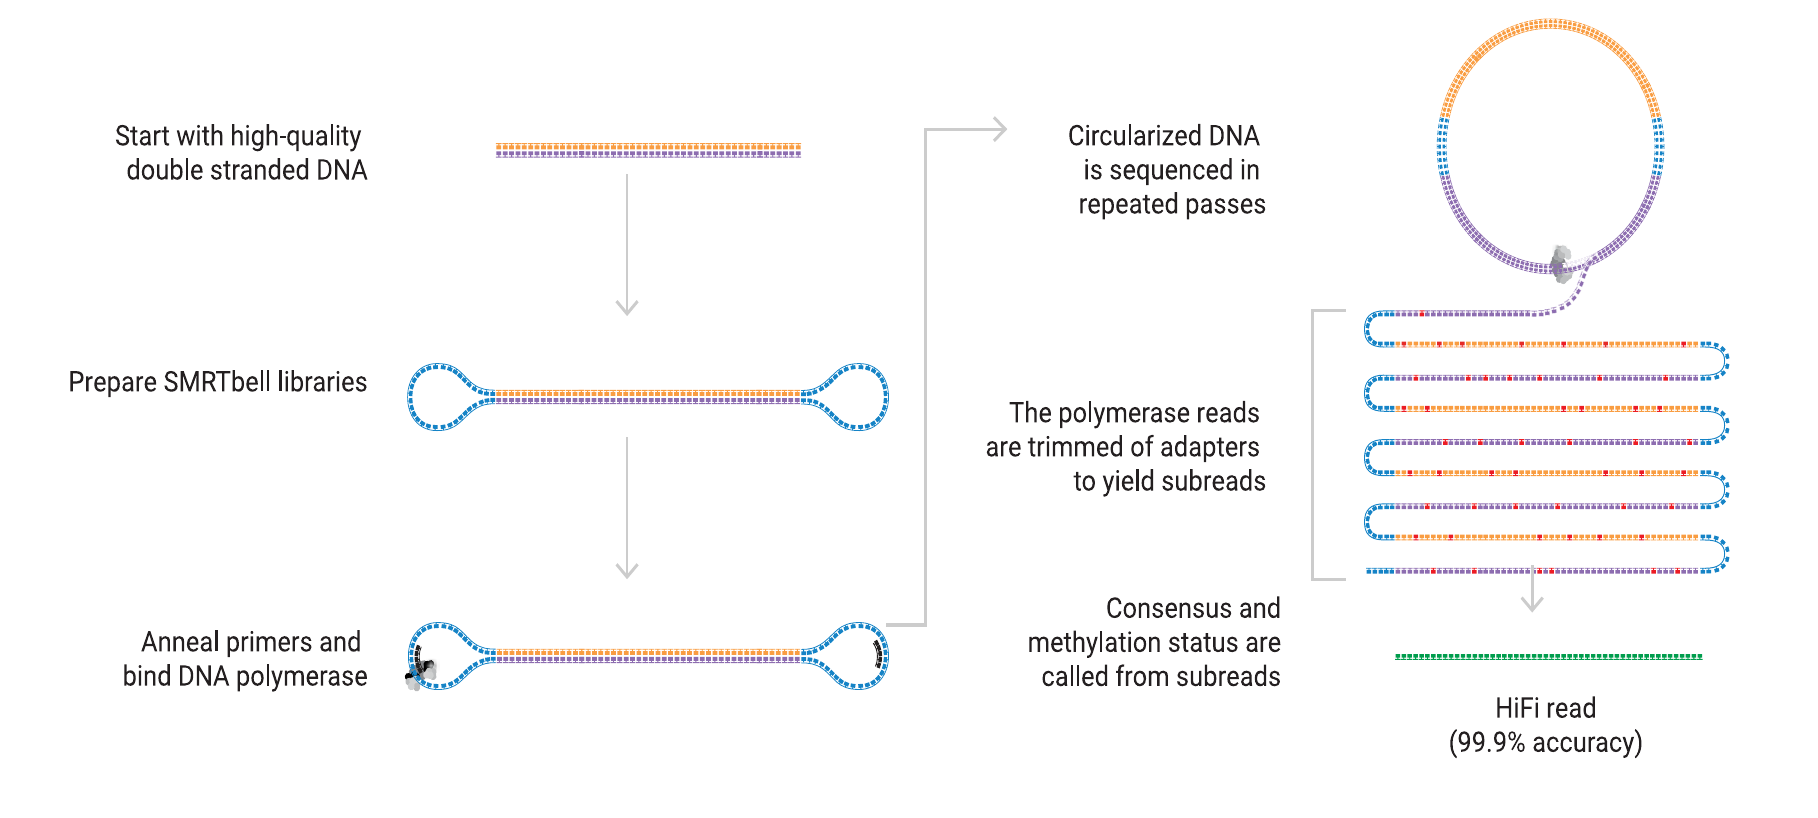
\includegraphics[width=0.95\textwidth]{figures/background/hifi_pacbio.png}
		\caption{Pacific Biosciences Hi-Fi reads generations scheme. Image from PacBio website.} 
	\end{subfigure}%
	\\
	\begin{subfigure}[b]{0.95\textwidth}
		\centering
		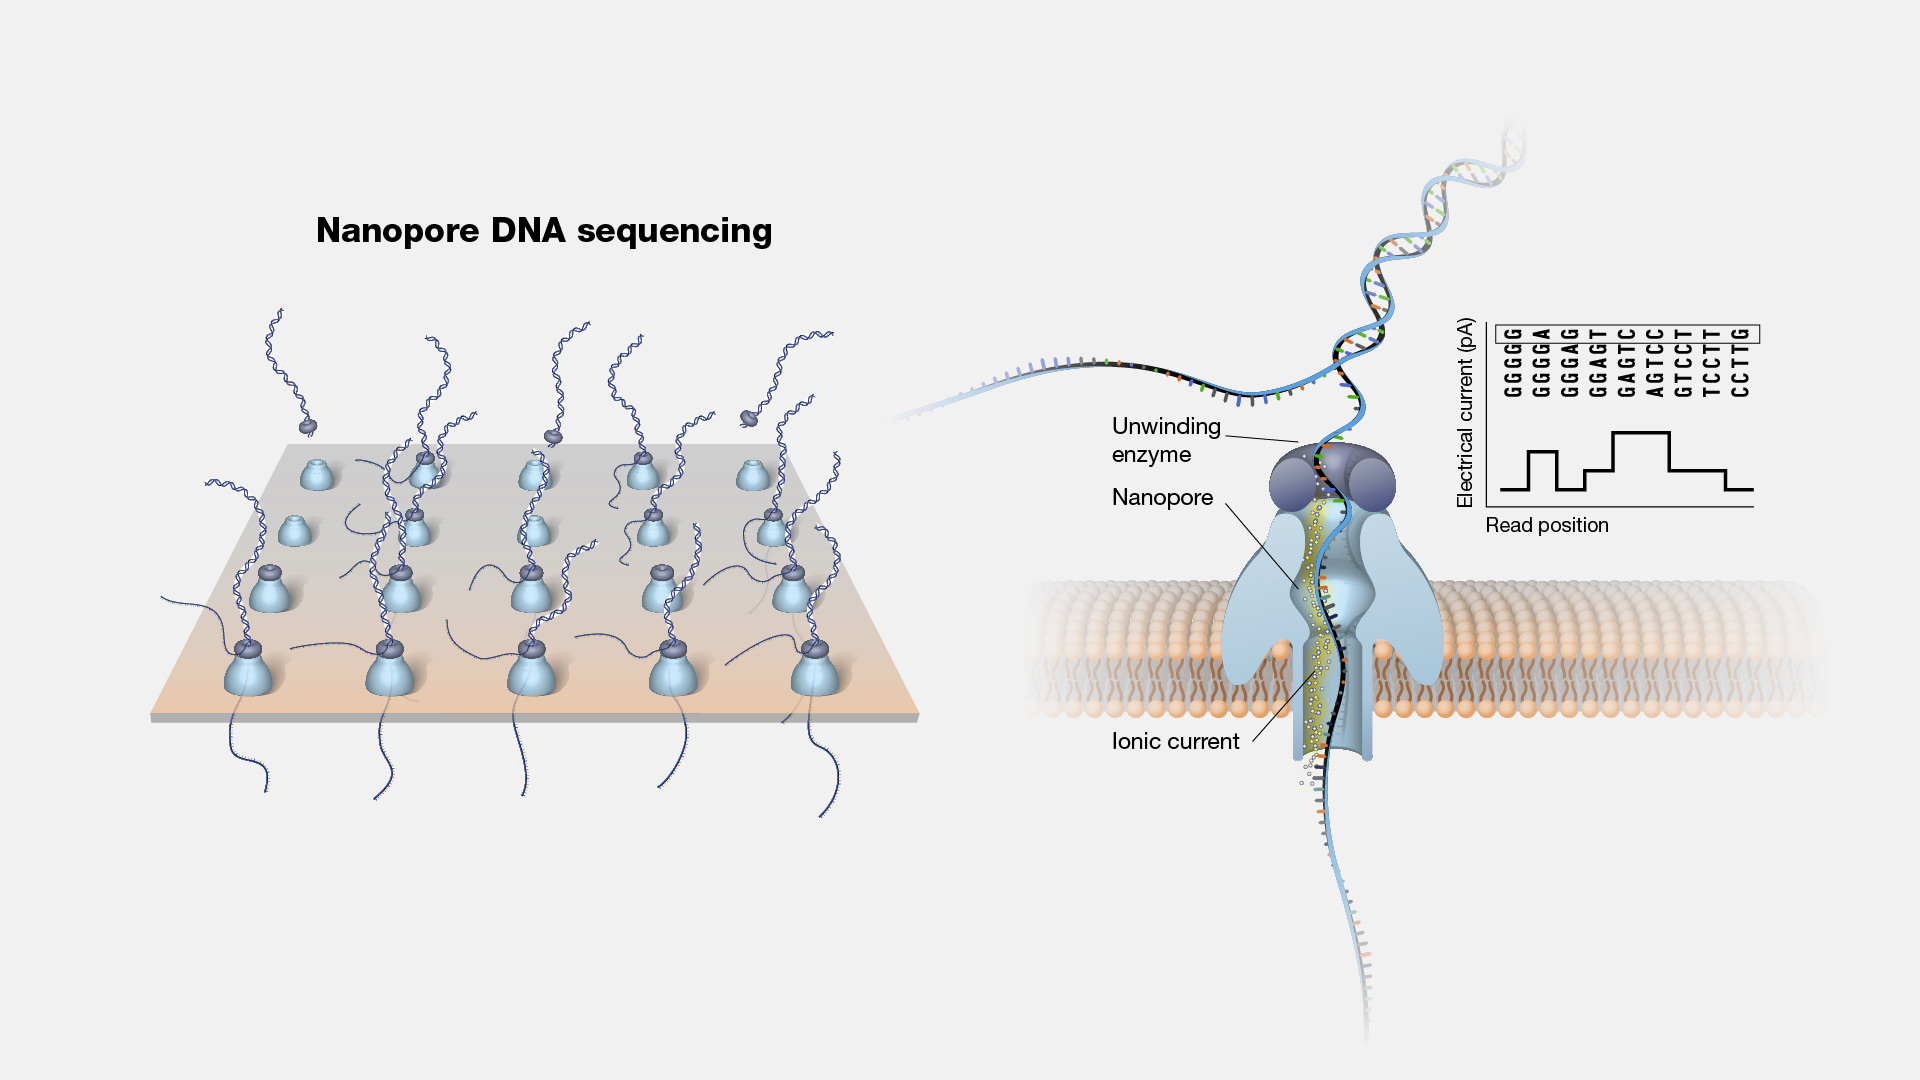
\includegraphics[width=0.95\textwidth]{figures/background/nanopore_sequencing.jpg}
		\caption{An array of pores sequences multiple molecules in parallel. A double stranded DNA (\gls{dsDNA}) molecule is split by the helicase enzyme and then a single stranded DNA (\gls{ssDNA}) sequence slowly gets through the pore for sequencing. Changes in the ionic current is used by a machine learning algorithm to infer the nucleotides of the sequence.} 
	\end{subfigure}%
	\caption{Third generation sequencing technologies.}
	\label{fig:sequencing_technologies}
\end{figure}

\section{From reads to \kmers and beyond}
\label{sec:kmer}
The sequences produced by any of the aforementioned technologies are considered as text strings, i.e. successions of characters, like the phrases of this manuscript, in which each character correspond to a nucleotide. These sequences can therefore being stored in plain text formats, like FASTQ, that preserve basecalling quality information or in others, like FASTA, that retains only the actual sequence. In order to use less space and take advantage of redundancy in the sequencing data, these files are often compressed, using one of the many tools publicly available like \texttt{gzip} or \texttt{zstd}, by Facebook. \\
As paired-end short-reads have different features than ultra-long reads or Hi-Fi long reads, most of the tools focus on providing applications for just one single type. In cases like assembling a genome from the reads or calling the variant of the sequenced genome compared to one reference, the information from different sources can be combined to provide superior results. In order to generate high-quality genome assemblies, for example, many consortia, like the Human Pangenome Reference Consortium, use Hi-Fi long reads as bases for assembly plus ultra-long reads as scaffolds to chain together the assemblies into sequences that span from telomere to telomere of a chromosome.\\
In the work presented in this manuscript, most of the tools will ingest as input or raw sequences (both NGS or TGS) or high-quality, near telomere-to-telomere assemblies. Some of the tools that I have used and all of the ones I have developed or co-developed transform the input sequences or assemblies into \kmers to produce the desired output. \\
\begin{description}
	\item[DNA alphabet] The DNA alphabet, denoted by $\sum$ consists of the four characters representing the first letter of the nucleobases: A,C, G and T: $ \sum = {A, C, G, T}$, 
	\item[sequence] a biological sequence from $\sum$ is defined as $ S \in \sum^{l}$, with $\lvert S \rvert = l $, with length $l$ of arbitrary length.
	\item[sequence read] a read is a biological sequence obtained from sequencing. Its length, denoted as $z$, is tipically fixed, if generated by NGS, or variable, if produced by TGS.
	\item[\kmer] a \kmer of $S$, denoted as $x$, is defined as $ x \in \sum^{k}$, with $\lvert \kmer \rvert = k $ i.e. any valid sub-string of $S$ of length $k$. 
\end{description}
As shown in table~\ref{tab-kmers}, from any sequence $S$, it is possible to obtain its constituent \kmers. To efficiently extract all \kmers from a sequence, the best approach is to employ a sliding window technique. This is done by identifying the first \kmer at the start of the string and then iteratively shifting the window one position at a time, appending the newly encountered character to the right while removing the leftmost character.\\ The length $k$ of a \kmer is an arbitrary value, that is usually chosen depending on the kind of sequences used (cannot have $k$ > $n$, with $n$ the length of a the read from which it is derived), the characteristics of the data that is used (is it from a single organism, a collection of the same species, a collection of different organisms) and on the disk or memory space that is available for computation or storage (as in table~\ref{tab-kmers}, the longer the $k$, the more space is used by repeating the characters of the same underlying sequence in multiple \kmers). A more detailed explanation of these considerations will be provided in section~\ref{sec:qf}.\\
As it is possible to retrieve \kmers from a single read, it is trivial to extend this property to any set of reads, for example produced by a single sequencing run of a sample. This does not directly mean that a set of \kmers is not properly equivalent to the set of reads it is obtained from. In order to characterize this transformation as lossless, i.e. without any loss of information, an association from each \kmer to the read(s) it comes from would be needed. In most of the cases this is not useful and \kmers are obtained from reads without remembering from which reads do they come from. In other, specific, applications it might instead be needed to know in which reads there are certain \kmers~\cite{back_to_sequences}. %More considerations on this are going to be presented in section XXX[BackToSequences].\\
As presented in section~\ref{sec:dna} the DNA is double-stranded, with A bases are paired with T ones, while C bases are paired with G ones, also called complements. If a \kmer appears in a sequence, in the other strand of the molecule there would be what is called its reverse complement. This is the spelling of the \kmer from the end to the beginning, substituting each base with its complement. For example if in one strand there appear the sequence $ATGC$, on the other strand would spell $GCAT$.\\
When enumerating \kmers from a sequence or when storing them, only "canonical" \kmers are kept: this means that for each \kmer produced from a sequence, its reverse-complement is computed and only the one that is considered smaller by a certain property is kept. For example, if the lexicographic order is used, the \kmer (with $k=4$) $ACGT$ is lexicographically smaller than $TGCA$ so when either of the two is seen, only the first is kept.\\
A classic operation that is done when enumerating \kmers from sequences is to keep track of how many times each canonical \kmer appears in the set of sequences. This is called \kmer counting and finds important applications in many genomic disciplines like metagenomics or transcriptomics.\\
\kmers are being used in lots of applications based on NGS short reads while they are less applied on methods for error-prone long reads because using \kmers on one side destroys the long range information provided by reads that span thousands of bases, on the other error-rates higher than NGS would produce too many erroneous \kmers that would be very difficult to correct if not with very deep sequencing, providing additional cost bottlenecks. With Hi-FI reads and improved quality of Nanopore basecalling, it is possible to overcome the error limitation and use \kmers for long reads. One example that uses advanced concepts based on \kmers is the tool \mdbg that drastically improved assembly of Hi-Fi reads.\\ 

\subsection{\kmer based objects}
\label{sec:kmerobjects}
\textbf{Unitigs} correspond to the string spelled by concatenating a non-branching path in a \dbg, which is a graph representing the overlap between all unique \kmers from a set of sequences. In almost all applications unitigs are considered as maximal, i.e. the result of the maximum non-branching path in the graph. Non-branching paths are concatenations of nodes that have in-degree and out-degree of 1. The \dbg is more formally defined in section~\ref{sec:dbg_intro} \\
\textbf{Minimizers} are strings of fixed length that are used to subsample \kmers from sequences, since consecutive \kmers are overlapping and contain redundancy. The sampling is done by a pre-defined optimization function, with guarantees that the sampling will produce similar outcome from similar sequences. The function depends on the application and can be for example lexicographic order or the minimum value of a transformation (hence the word \emph{minimizer}). There are multiple declinations of minimizers. The first distinction is on the way they are chosen: on a sliding window or the 'universe'. When minimizers are chose on a sliding window of length $w$, every \kmer is evaluated against the chosen function and each $l$ character the one with the best value is retained. Universal minimizer are instead chosen independently of any spacing in the sequence and are the ones whose output value of the defined function is, for example, smaller than a threshold. \\
Minimizers can be also used as smaller subsequences of length $m < k$ inside \kmers to help group together \kmers based on their corresponding minimizer. In this case from each \kmer the \emph{m-mer} that minimizes the function will represent it. \\
\textbf{Super\kmers} are strings produced by concatenating adjacent \kmers sharing the same minimizer. They reduce the redundancy of consecutive \kmers and decrease the amount of data needed to represent a set of \kmers. 
\begin{table}[!ht]
	\begin{center}
		
		\begin{tabular}{ c c c c c c c c c c c}
			\toprule
			Position & 1 & 2 & 3 & 4 & 5 & 6 & 7 & 8 & 9 & 10 \\
			\midrule
			Sequence $S$ & C & T & G & A & A & C & T &A & C & A\\
			\midrule 
			$3-mers$ & C & T & G  \\
			&   & T & G & A \\
			&   &  & G & A & A \\
			&   &  &  & A & A & C\\
			&   &  &  &  & A & C & T\\
			&   &  &  &  &  & C & T & A \\
			&   &  &  &  &  &  & T & A & C \\
			&   &  &  &  &  & & & A & C & A\\
			
			\hline
		\end{tabular}
		
		\vspace*{0.3 cm}
		
		\centering
		\begin{tabular}{ c c c c c c c c c c c}
			\toprule
			Position & 1 & 2 & 3 & 4 & 5 & 6 & 7 & 8 & 9 & 10 \\
			\midrule
			Sequence $S$ & C & T & G & A & A & C & T &A & C & A\\
			\midrule 
			$4-mers$ & C & T & G & A \\
			&   & T & G & A & A\\
			&   &  & G & A & A & C\\
			&   &  &  & A & A & C & T\\
			&   &  &  &  & A & C & T & A\\
			&   &  &  &  &  & C & T & A & C\\
			&   &  &  &  &  &  & T & A & C & A\\
			
			
			\bottomrule
		\end{tabular}
		\caption[\kmer computation from a sequence]{\kmers with $k=(3,4)$ being computed from the sequence \texttt{S} = \texttt{CTGAACTACA}. $l-k +1$ \kmers are generated for a total of $(l -k + 1) * k$ bases. While with $k=3$ the total bases are $ 8 * 3 = 24$, with $k=4$ they are instead $28$, as larger $k$ encodes more information redundancy.}
		\label{tab-kmers}
	\end{center}
\end{table}


\begin{table}
	\begin{center}
		\begin{tabular}{c | c}
			
			Sequence id & sequence \\
			\hline
			seq1 & ACATCA \\
			seq2 & CTTCAG \\
			seq3 & TACAGC \\
			seq4 & GCTTAC \\
			
		\end{tabular}
		\newline
		\vspace*{0.2 cm}
		\newline
		
		\begin{tabular}{c | c | c | c  | c}
			
			Sequence id & seq1 & seq2 & seq3 & seq4\\
			\hline
			\kmers  & \underline{ACA} (TGT) & CTT (\underline{AAG}) & TAC (\underline{GTA}) & GCT (\underline{AGC}) \\
			& CAT (\underline{ATG}) & TTC (\underline{GAA}) & \underline{ACA} (TGT) & CTT (\underline{AAG}) \\
			& \underline{ATC} (GAT) & \underline{TCA} (TGA) & \underline{CAG} (CTG) & TTA (\underline{TAA}) \\
			& TCA (\underline{TGA}) & \underline{CAG} (CTG) & \underline{AGC} (GCT) & TAC (\underline{GTA}) \\
		\end{tabular}
		\newline
		\vspace*{0.2 cm}
		\newline
		
		\begin{tabular}{c | c}
			
			ordered canonical \kmer & count\\
			\hline
			AAG & 2 \\
			ACA & 2 \\
			AGC & 2 \\
			ATG & 1 \\
			ATC & 1 \\
			CAG & 2 \\
			GAA & 1 \\
			GTA & 2 \\
			TAA & 1 \\
			TCA & 2 \\
		\end{tabular}
	\end{center}
	\caption[Example of canonical \kmer counting.]{Example of canonical \kmers enumeration and count. Given a set of sequences, for each of them \kmers are computed in a stream. For each of them, on the fly, the reverse complement is computed. Then the ones that are considered canonical are passed and counted.\\ Reverse complements are between parentheses and the canonical between the two (by lexicographic order) is underlined.}
	\label{tab-lista-kmer}
\end{table}

\clearpage

\section{Genetic diversity: focus on humans.}
\label{sec:background_pangenomics}
%Genomic variations are the characteristics that produce differences between organism of a species or between species. 
The Human genome contains more than 3 billions base pairs and includes 42,611 genes, of which 20,352 are presumed protein-coding genes, i.e. specific sections of DNA that serve as blueprints for proteins. The remaining 22,259 are non-coding: they produce RNA that serves a biological function but that it is not translated into proteins~\cite{chess}. The rest of DNA consists of regions that function as regulatory element, like enhancers, promoters and silencers or as other conserved, functional element. Variations in specific regions cause phenotypic changes that can increase, decrease or not affect the fitness of an individual.\\
Genetic diversity is the variability that exists between organisms at the genetic level, i.e. differences in the information enclosed in their DNA. It is the raw material for biological evolution as, without heritable genetic differences between us, we would not be able to biologically evolve. Here what I will present is valid for humans, as the large part of my work has been with human DNA sequences. Most genetic changes have no effect on the individuals carrying them but some can result in phenotypic differences.\\

\subsection{Causes and drivers of genetic diversity in humans}
There are two main mechanisms of genetic diversity: the arise of new mutations and the reshuffling of already present genetic material trough recombination and duplications. Mutations can arise through two processes. First, if physical or chemical damage, such as caused by UV radiation, occurs prior to cell division and is not repaired, a wrong base can be integrated in the DNA of the cell. Second, errors during the DNA replication in cell division can lead to mutations. When this occurs in germinal cells they are transmitted to the offspring, while when happening in a somatic cell (not reproductive), the mutation is not transmitted but can instead be responsible for certain type of cancer. In humans, it is estimated that a newborn carries on average 70 point mutations (one nucleotide substitute with another), 15 from the mother and 55 from the father. The amount of mutations is proportional with the age of the person and, more than induced by replication, it is due to not corrected damage.\\
On top of the mutations, chunks of chromosomes from the mother and the father chromosomes are shuffled to produce new combinations. The effect of this random process produces the differences between siblings with the same biological parents. Recombination is heterogeneous in the DNA and depends on some motifs that promote higher recombination. Finally, recombination is also influenced by the age, mostly of the mother, as older mothers tend to produce offspring with more misplaced recombinations, also causing the well known trisomy 21.\\
Without diverging too deep into population genetics, it is also important to understand how new variations are conserved, lost or fixed (become prevalent) in a population. These outcomes are driven by two main factors: genetic drift and natural selection.\\
Genetic drift is a process, given by the randomness in the individuals that reproduce in a specific population. This can contribute to the loss or fixation of some variants just because of randomness and not because they provide an advantage to the individual. Specifically, in populations with small number of reproductive individuals, this can fixate detrimental variants, while in large populations, the large number of individuals buffers the event. \\
Natural selection, on the other hand, is a mechanism that explains human evolution: as genetic variations causes the gain or loss of specific phenotypic traits, these traits can confer positive or negative advantage compared to the rest of the individual in a population (fitness). This phenomenon can contribute selecting certain variations in a population by either contribute to the fixation or the loss of a variant. This mechanism explains our species adaptation to nutritional resources, climate and pathogens: in 10 thousand years a mutation in a gene that conferred the ability to digest milk as adults, the lactase persistence, applied such a strong selective pressure that has almost reached fixation in some human populations (mostly of North-European or African ancestry)~\cite{lactase}. Selection on certain genes explains better adaptations to cold or high altitudes and selection in HbS or DARC alleles has helped humans adapt and survive malaria infections\cite{genome_diversity_quintana}. 
\subsection{Human Genomic variation: types of variants}
There are various types of genomic variants: from the shortest, the single-nucleotide variants (SNV) or Single Nucleotide Polymorphism (SNP) when it is present in at least 1\% of the population, is the difference of one nucleobase between two individuals. In a specific part of the genome one person can have instead of a cytosine (C) a thymine (T), like for the SNP located 14 thousands bases upstream of the lactase gene that enables the lactase persistence mentioned earlier\cite{lactase_persistance}.
A second group of small variants is made of insertions and deletions (called together \emph{indels}): these are events in which it is present or missing a group of less than 50 nucleotides. The number of nucleotides is an arbitrary threshold used to better separate them from other kind of variations. Specific types of indels are the tandem repeats that, as the names suggests, are insertions or deletions of small repeated sequences of DNA. These repetitions usually are one after the other with no other sequence in between~\cite{nih_variation}.\\
\begin{figure}[!ht]
	\centering
	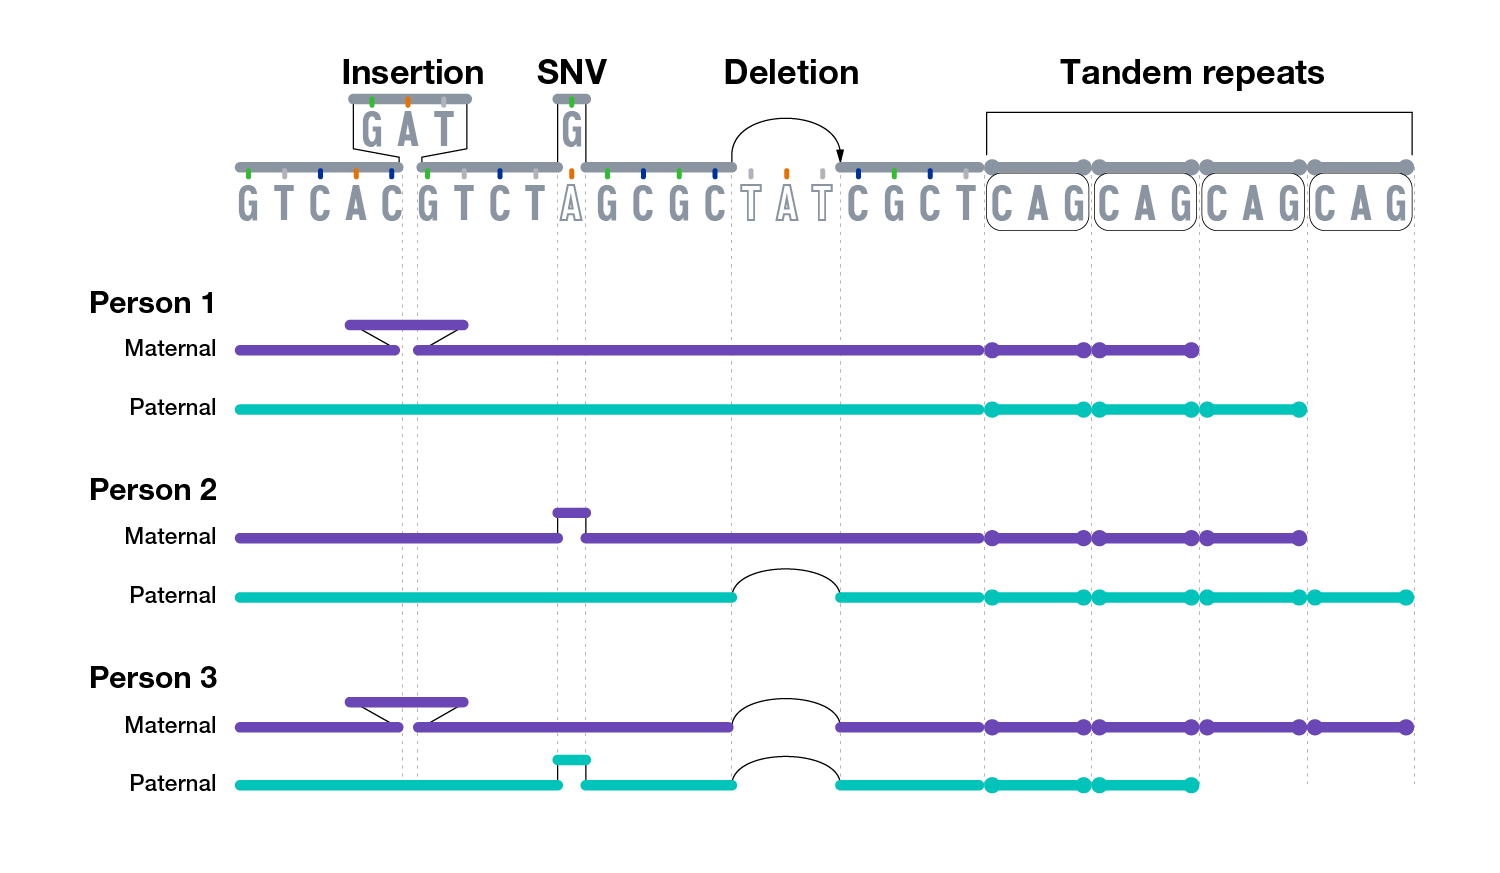
\includegraphics[width=\linewidth]{figures/background/small_variants.png}
	\caption[Small genomic variants.]{Graphic showing the types of small genomic variants~\cite{nih_variation}. Individuals have different genomes, and these differences are encoded as variations in their DNA sequences. The most common type of variation between individuals is a Single Nucleotide Variation (SNV), in which a base at a specific position is different (e.g., A and G). Another common variation is the presence of extra or missing nucleotide(s) in a specific part of the DNA: when this difference involves fewer than 50 nucleotides, it is called an insertion or deletion (INDEL). Finally, tandem repeats are contiguous repetitions of a small stretch of nucleotides.\\ In this example Person 1 has an insertion in the Maternal haplotype and a different number of repetitions of \texttt{CAG} in the tandem repeats. These are referred to as heterozygous variations because they differ in their form between the two chromosome copies.\\ Person 2 has an SNV in the maternal haplotype, where the base G appears instead of the more common A. In the paternal haplotype,  the \texttt{TAT} sequence is deleted, while the number of \texttt{CAG} repeat copies is different: with four on the paternal haplotype and three on the maternal chromosome. \\ In the case of In the case of Person 3, a deletion is present in haplotypes.}
	\label{fig:small_variants}
\end{figure}
These groups of small variants, shown in figure\ref{fig:small_variants} are the most described, studied and associated with diseases as they were the only one consistently detectable with NGS sequencing. For these reason, studies that tried to associate genomic variation with diseases commonly used only these kind of variants.\\
The other kind of variations are the ones that stretch at least 50 nucleobases and that can reach the dimension of large chunks of the chromosomes: they are called structural variations (SVs).
These can be indels or tandem repeats with the repeated section longer than 50 nucleotides, accounting for nearly half of all SVs, that take the name of Copy Number Variants (CNVs). Moreover, there are also inversions, in which a chunk of DNA is inverted compared to another and translocations in which pieces of two different chromosomes trade places~\cite{nih_variation}.\\
\begin{figure}[!ht]
	\centering
	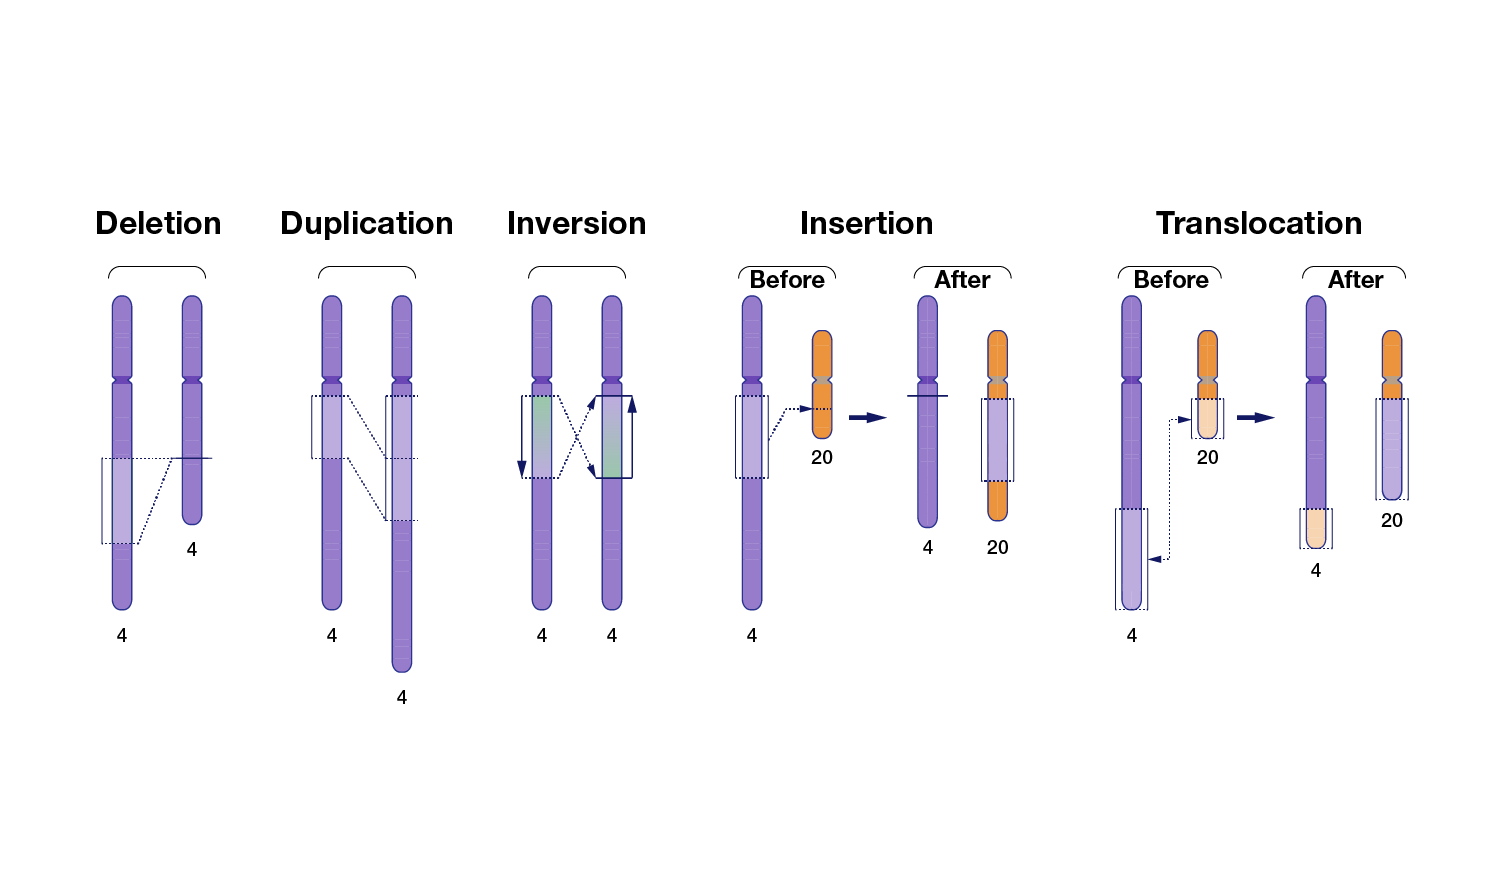
\includegraphics[width=\linewidth]{figures/background/large_variants.png}
	\caption[Large genomic variants.]{Graphic showing the types of large genomic variants, also named structural variants~\cite{nih_variation}. Deletion or insertions of more than 50 base pairs are considered structural variants.\\ Duplications are when large segments are copied one or multiple times. They tend to have a nested and modular structure. The copies can span non-coding regions or genes. Different copies of genes can alter the expression of the associated protein. This is not the case for gene TBC1D3, a primate-specific gene associated to increase of the prefrontal cortex. The high variability in the human population for such an important gene has been recently explained by the fact that the expression is limited to a subset of copies~\cite{tbc1d3}.\\  An inversion is a segment of a chromosome that preset in the reverse orientation as a result of breaking off and errors in the reattachment. Inversion can be cause diseases, like hemophilia A, or increase the risk of further mutations that can cause disease, like for the microdeletion syndrome~\cite{inversions_disease}.\\ A translocation occur when a chromosome breaks and a portion is attached to another chromosome: this event can cause diseases like leukemia~\cite{leukemia}. }
	\label{fig:large_variants}
\end{figure}
Finally, it is important to remember that these kind of variations can be on just one haplotype (copy of the chromosome) or on both. An heterozygous allele is referred to having inherited from the mother and father a different version of a specific part of the genome.

\subsection{The importance of studying genomic diversity in populations context}
DNA differs between individuals of the same population (inter-individual) and between different populations of the same species (inter-population): figure~\ref{fig:pop_diff} shows the percentage of inter-individual variation for four close primates. Different species may vary in the amount of genetic diversity present between individuals within a population, as seen in humans, or between populations, which accounts for a significant portion of genetic variation in orangutans. As discussed before, differences in DNA are given by having a different nucleotide at the same place (SNV), indels and large and complex variations, up to Megabases, that can produce different counts of copies or different ordering of a same region. \\
On average, each human carries around 10 thousands amino-acid altering mutations, 300-400 gene disruption events (like stop, splice and indels) affecting 200-300 genes and is heterozygous at 50-100 mutations associated with an inherited disorder~\cite{genome_diversity_quintana}. 
Finally, even when close species share a large portion of genetic material, structural changes that rearrange the same material in different order or invert it, contribute to meaningful changes. In figure~\ref{fig:chromosome_diff} it is shown how the chromosome 7 and 16 of some primates, even if very similar, differs in terms of organization. These large structure rearrangements are thus fundamental to understand the biology of organisms.

Moreover, genetic diversity is driven by two main factors: genetic drift and natural selection. Genomic duplication followed by adaptive mutation is considered one of the primary forces for evolution of new functions~\cite{tbc1d3}.
\begin{figure}[!ht]
	\centering
	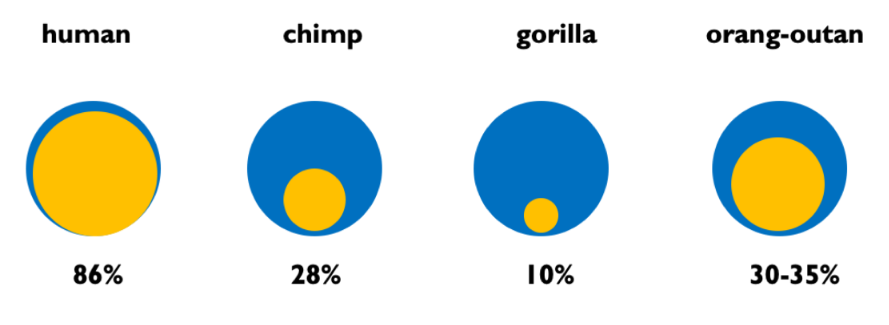
\includegraphics[width=.8\linewidth]{figures/background/pop_diff.png}
	\caption[Inter-individual and inter-population variation for 4 primate species.]{Share of inter-individual (yellow) and inter-population (blue) diversity for four different primates. While for humans the  majority of the diversity is within populations, for other primates it is between populations. This shows how Humans are more mixed than other primates. Percentage shows the inter-individual variation share~\cite{genome_diversity_quintana}.}
	\label{fig:pop_diff}
\end{figure}

\begin{figure}[!ht]
	\centering
	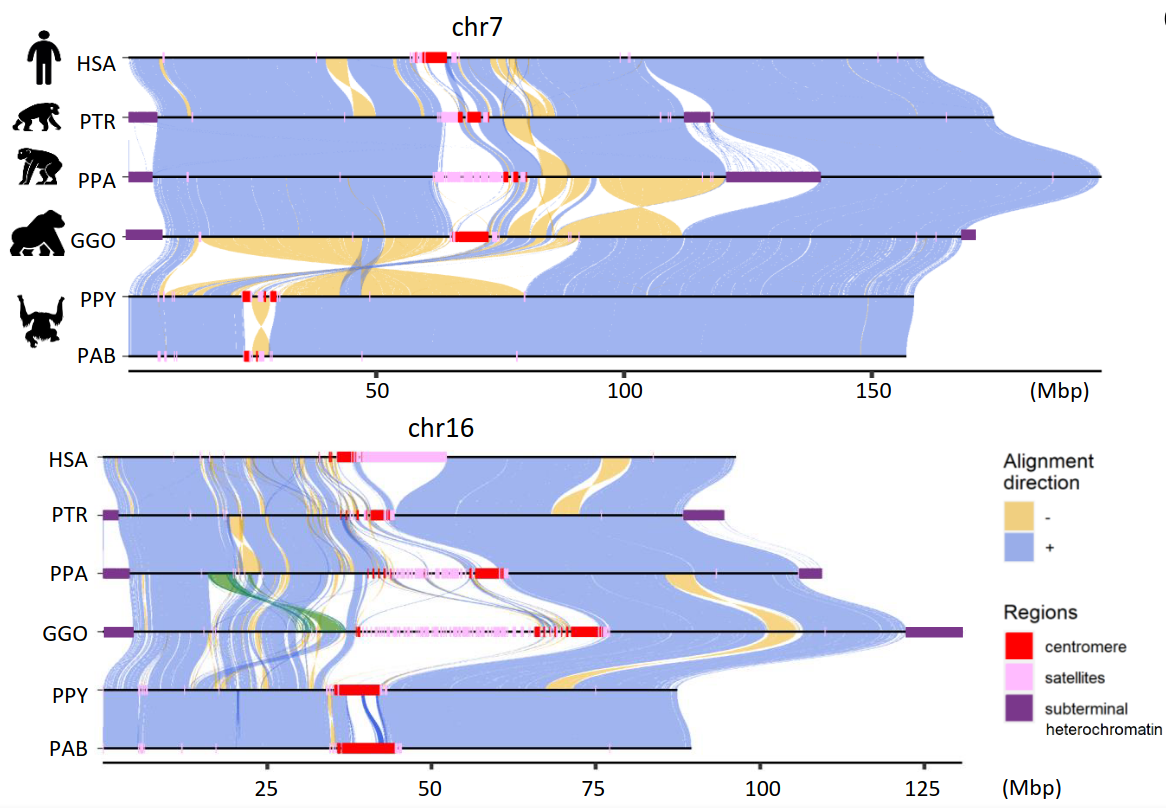
\includegraphics[width=\linewidth]{figures/background/genome_diff.png}
	\caption[Genomic difference in chromosome 7 and 16 of 5 primate species.]{A comparative ape alignment of human (HSA) chromosomes 7 and 16 with chimpanzee (PTR), bonobo (PPA), gorilla (GGO), Bornean and Sumatran orangutans (PPY and PAB). The image on the top shows most of the chromosome 7 is conserved except for large inversions happening between the species. The image below shows complex inversions in chromosome 16. Image taken from "Complete sequencing of ape genomes"~\cite{ape_genomes}.}
	\label{fig:chromosome_diff}
\end{figure}

\begin{figure}[!ht]\clearpage
	\centering
	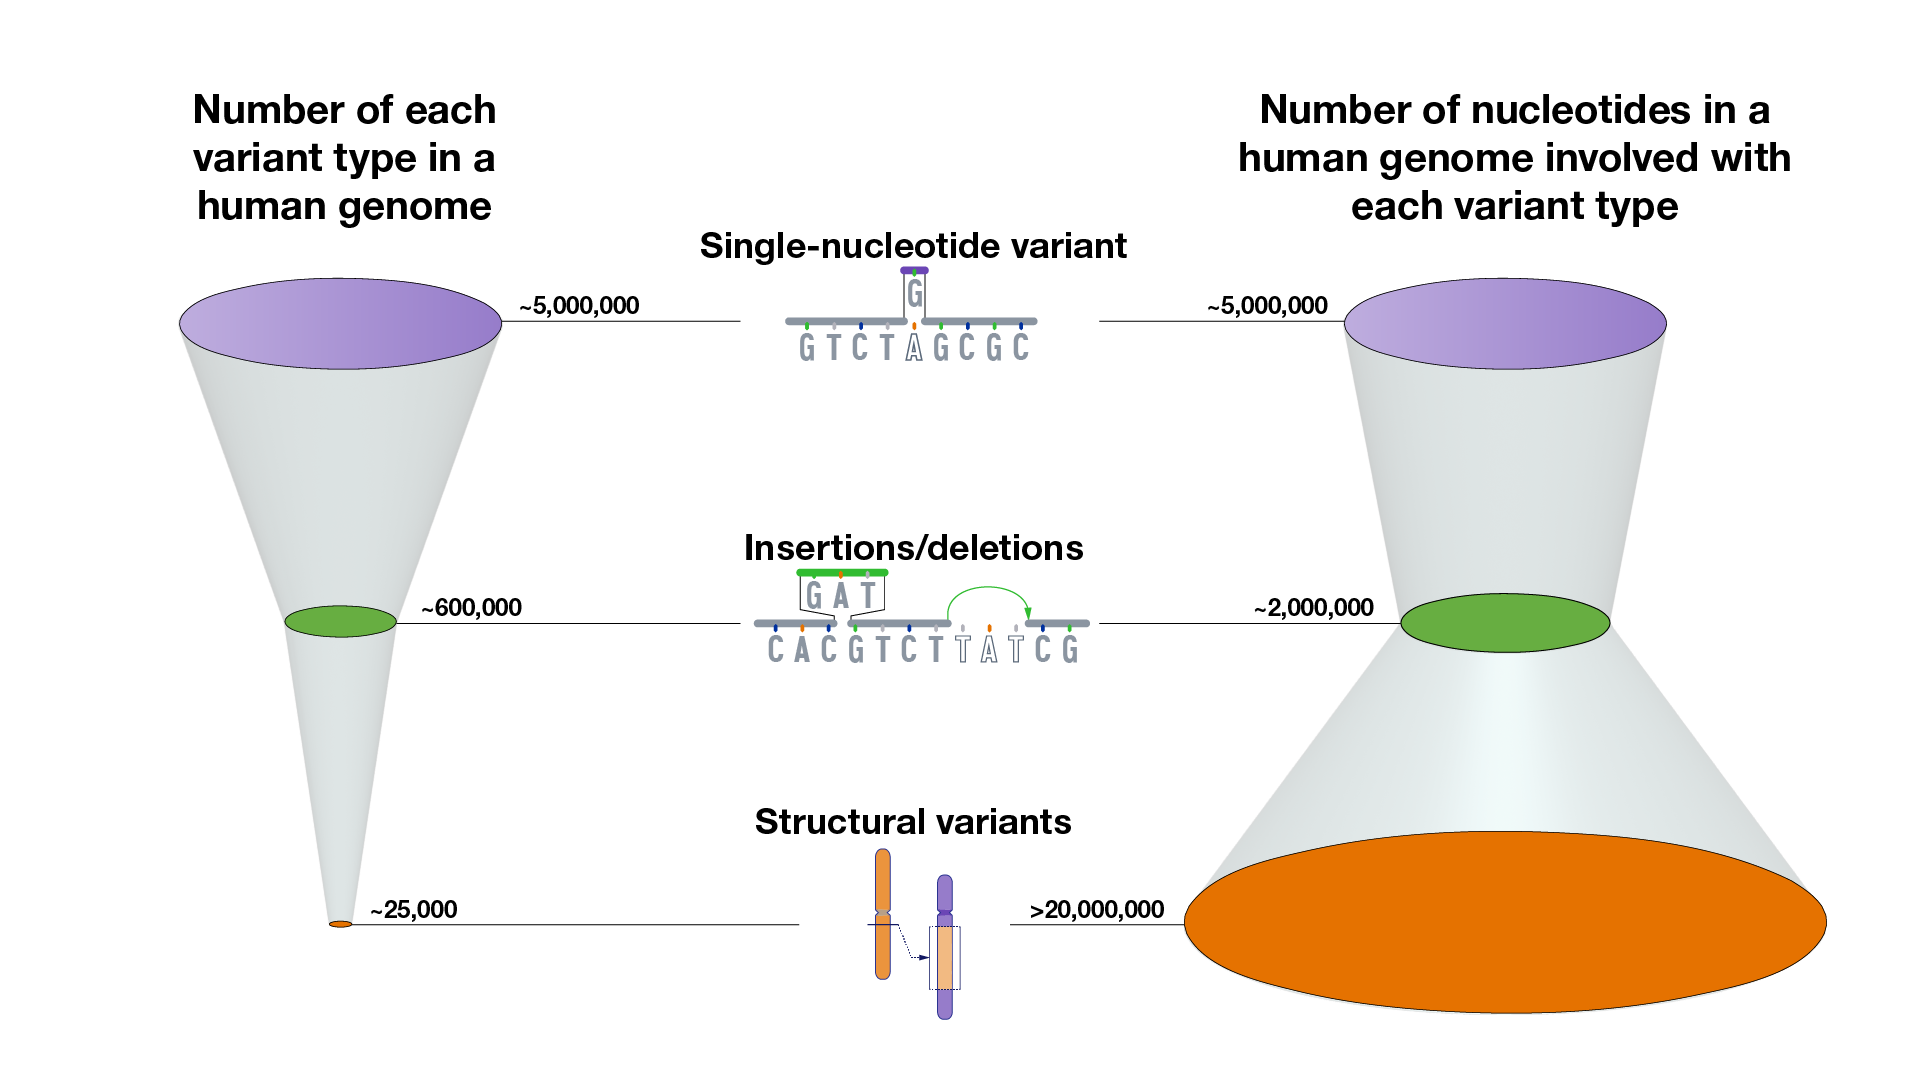
\includegraphics[width=.95\linewidth]{figures/background/genomic_spectrum.png}
	\caption[Spectrum of Human Genetic Variation.]{Spectrum of Human Genetic Variation~\cite{nih_variation}. While SNPs are the most common variation event, their impact in the total amount of bases in a genome is $\sim4$ times smaller than the one of Structural Variations, that are 200 times less frequent. This shows the great need to consider SVs in genomic analysis and not to stop at the SNP/indel level.\\}
	\label{fig:variation_spectrum}
\end{figure}

\section{Pangenomics, pangenomes and pangenome graphs}
\subsection{The premises for Pangenomics}
There are a number of factors that must be taken into consideration to understand one side the need for a new paradigm and on the other side the conditions that lead to its development. Here I will briefly expose some of them before diving into pangenomics approaches and methods. 
\subsubsection{A single linear genome for all analyses}
Since the first complete genome sequences have been available in the late '90, all analyses based on sequencing data depended upon the use of a single linear reference genome, i.e. the best version of the genome available for any species. This reference sequence can originate from the genome of a single organism or be a patch and consensus of multiple available genomes of the same species. Its purpose is to use it infer information from newly, less refined, genomes that are being sequenced. We now know that this approach is suboptimal in a wide range of applications as a lot of genetic material of the species cannot be present in a single linear representation: this is valid for eukaryotes and even more for bacteria, that tend to be very diverse even in the same strain. The goal would therefore be to find a representation that provides more genetic material of a single species by intelligently combine the information from genome of multiple organisms and their differences.

\subsubsection{A quantity and quality revolution }
In the last few years we are witnessing a new revolution in sequencing. As the price of sequencing is lowering more than 2x per year, from 1\$/basepair to \$$10^-7$/basepairs\cite{durbin_recomb}, new scientific discoveries and technological advances are leading to a remarkable increase of quality, in term of per-base error rate, and throughput of TGS. This means that in the next future we will dispose of a rich wealth of high quality sequencing information to produce hundreds or thousands of new first grade assemblies of large eukaryotic genomes. 

%This limitation at the beginning was not solvable due to the scarcity of high quality assembled genomes as the technologies of sequencing and computational tools were not mature enough.

For example, the history of complete human genome assemblies clearly exposes how much more high quality genomes it is now possible to generate. The Human Genome Project took 13 years to produce its result~\cite{humangenomeproject} and the absence of long reads with low error rate made it impossible to automatically resolve repetitive regions like telomeres and centromeres~\cite{human-pangenomics-era}, producing a reference only $92\%$ complete~\cite{t2t}. This problem was only solved in 2022 with a new, reference genome that did not have any gaps or unresolved regions, from the telomere to the other telomere of each chromosome~\cite{t2t}. Now, many consortia are producing increasingly more genomes to a level comparable to the one produced in 2022. For example, the HPRC, i.e. the Human Pangenome Reference Consortium, released 47 new human genomes (92 haplotypes) in 2021 and has recently released other 153 genomes to a total of 400 haplotypes of very high quality.

Finally, it is important to understand the quantity of biological information produced. As shown in table~\ref{tab:bp-increase}, the number of base pairs sequenced has more than doubled each year since 1995. As this is faster than the famous Moore's law on computing power, it is becoming evident that a new paradigm is needed to store and analyze such wealth of data. Public repositories, like Sequence Read Archive (SRA) and European Nucleotide Archive (ENA), are rapidly increasing the number of samples being sequenced and rendered publicly available to everyone, with tens of billions of millions of basepairs from genomic samples, as shown in figure~\ref{fig:SRA}. Other repositories of genomic data with associated medical metadata, like the UK biobank that comprises around 500 thousands individuals, are also emerging. These conditions are pushing the adoption of novel methods to process and analyze genomes.

\begin{table}[!ht]
	\centering
	\begin{tabular}{c | c | c}
		year & genome(s) & base pairs \\
		\hline
		1995 & Bacterium & $ 2*10^6$ \\
		2001 & Mammal & $ 3*10^9$ \\
		2013 & 2500 humans & $ 7.5*10^12$ \\
		2021 & ~1M genomes & $ 3*10^{15}$ \\
	\end{tabular}
	\caption[Scale of DNA data increase over the years.]{Scale of DNA data increase over the years. Sequenced base pairs are now $10^9$ times compared to 30 years ago. The amount of data available more than doubled each year in the last $\sim30$ years. The rate was derive from $ \log_2(10^9) = 29.9 \implies 10^9 \approx 2^{30}$.\cite{durbin_recomb}.}
	\label{tab:bp-increase}
\end{table}
\begin{figure}[h!]
	\centering
	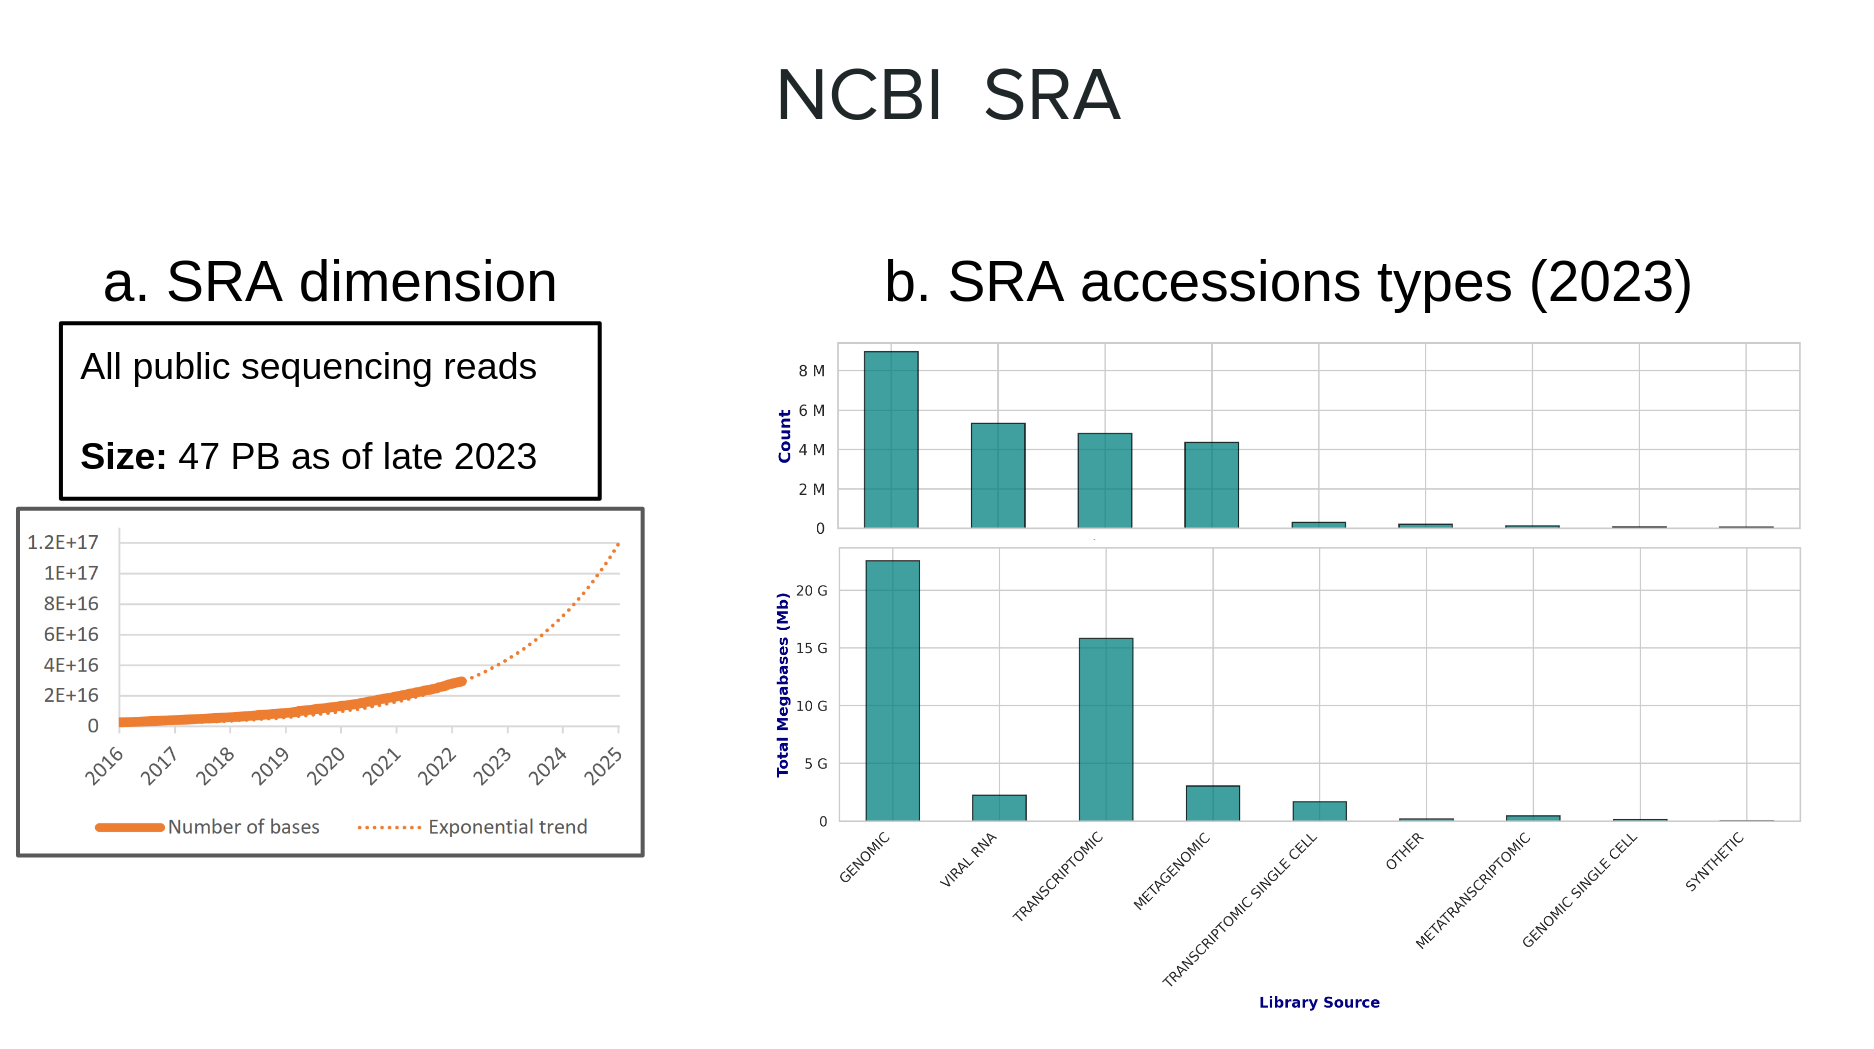
\includegraphics[width=\linewidth]{figures/background/sra.png}
	\caption[The Sequence Read Archive.]{a) The size in petabases (peta = $10^{15}$) of the SRA archive; b) The type of data in the SRA database shows the vast amount of genomic data available. Image made from Rayan Chikhi's slides.\\}
	\label{fig:SRA}
\end{figure}

\subsubsection{The need to better understand difference between genomes}
The ability to produce such good data is the main enabler of increasing efforts from the scientific community to propose new methods to analyze genomes: not anymore by comparing new genomes against a single good reference sequence but by comparing it in a comprehensive representation of the species. \\
Moreover, as new high quality sequences and assembled genomes are available, complex and/or highly repetitive regions can be now represented also for new genomes therefore enabling comparison between the ones of different genomes. This is very important as up until these improvement in sequencing and assemblies arrived, analyses were mostly blind to large, complex and/or repetitive structural variations. As we now know that these are the ones responsible for most of the difference between human genomes, new proposed approaches should provide new and better tools to understand, represent and analyze such variations.\\
Finally, as a single reference sequence cannot enclose all the possible structural variations of a population into a linear model, the need for a change in data structure for genomics arises.

%This novel way to overcome the limits of "linear genomic" and consider all the variation in a single species is called pangenomics. \\
%Various efforts are being made on producing reference pangenomes of yeasts, bacterias, plants and animals, including humans. In order to do so, new tools to construct and then analyse and use such representations are being developed. 
%It is important here to notice, as it will be stressed in the next sections and chapters, that construction is just the first step and that is very important to understand and work on which are the operations that can be succesfully performed by these representations. \\

\subsection{Pangenomics}
Pangenomics is a rapidly evolving field in genomics that aims to capture and analyze the full genetic diversity within a species or a group of closely related species. Unlike traditional approaches that rely on a single, linear reference genome, pangenomics compares genomes to a collection of others, representing all genetic variations and structural differences across a set of genomes. It leverages large collections of high-quality assemblies from many individuals or species to overcome the observational bias inherent in using a single haplotype as a reference for an entire population. As illustrated in Figure \ref{fig:pangenomics_model}, the pangenome model strives to represent all variations among a group of complete genomes by describing their direct relationships, whereas the linear model compares each genome only to a reference. While traditionally in genomics genomes were indirectly compared through their differences relative to a single linear reference, pangenomics enables direct comparisons between genomes. When a new genome is added to the collection, traditional genomics compares it solely to the reference genome, whereas in pangenomics, it is compared to all genomes in the model.
\begin{figure}[h!]
	\centering
	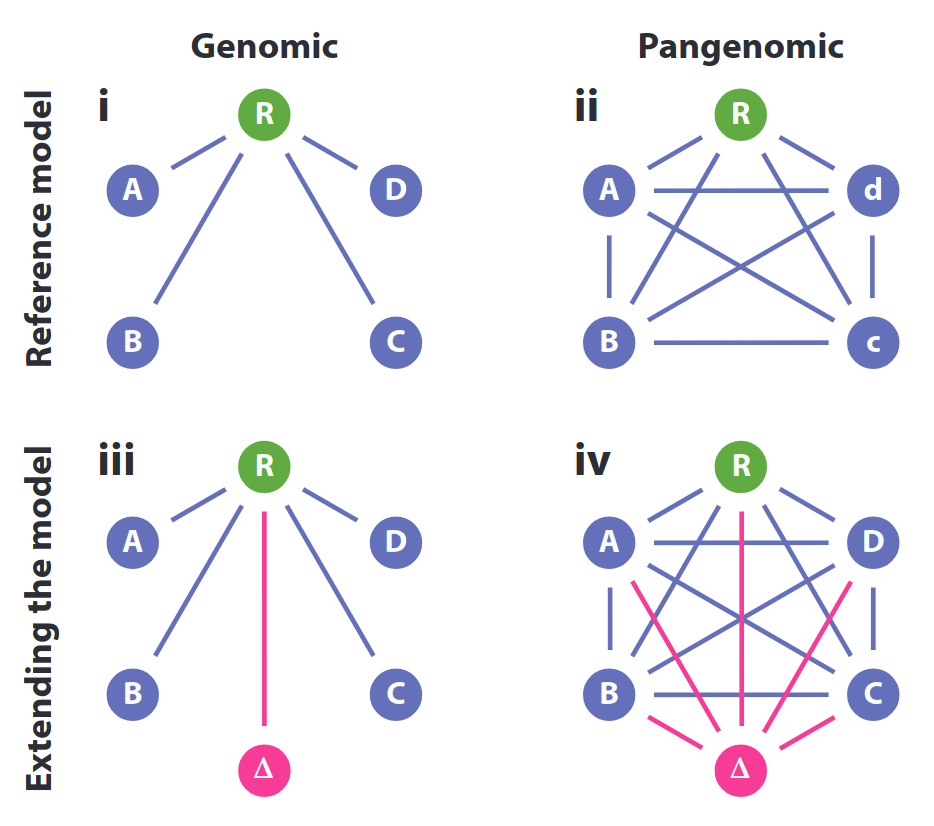
\includegraphics[width=.75\linewidth]{figures/background/pangenome_model.png}
	\caption[The Pangenome model.]{The genomic vs pangenomic model i) In the genomic model each genome is compared only to the reference sequence. Any comparison between a pair of genomes is done indirectly via their difference with the reference. ii) In the pangenomics, variations are described in a relative way for any genome. Any pair of genomes can be compared directly. iii) In the genomic model, to add a new genome in the collection it has to be compared to the reference. iv) In pangenomics, each new genomes added to the model is automatically compared to all the ones in the collection. Figure from~\cite{eizenga}\\}
	\label{fig:pangenomics_model}
\end{figure}
It was first conceptualized for bacterial genomes, and at gene level, without considering non coding regions. This was mostly due to the fact that bacteria share genes between each other, generating high diversity in the gene repertoire between organisms of the same species or strain.
The first proposed pangenome model had a subdivision between a core genome, made by genes present in all individuals of a species, and a dispensable or accessory genome, with genes present in some, but not all, individuals.\\
This definition would then extend to a more general model that would consider variations at the nucleotide level to contain all variations in a set of genomes.\\
\subsubsection{Pangenomes}
A pangenome can therefore be considered as any collection of genomic sequences to be analyzed jointly or to be used as reference. This definition provides two important concepts for the rest of the studies provided in this manuscript: 
\begin{itemize}
	\item[\textbf{Model}] The pangenome is not a well-defined structure or model; it can range from a simple collection of sequences to more complex data structures. As a result, various approaches have been developed and are employed depending on the specific application or research focus.
	\item[\textbf{Scope}] a pangenome can be either used as:
	\begin{itemize}
		\item A new reference for a specific species to be used for analyses in a similar way as linear genome. This means that a large consortium would be producing a representation that is accepted as new standard. For the Human genome this is done by the HPRC consortium as the T2T consortium produced the best-quality linear reference genome~\cite{t2t}.
		\item A different model that can be used to study a set of genomes, without needing \emph{a priori} to use a reference. This model can find applications in population variation studies. 
	\end{itemize} 
\end{itemize}
A pangenome can also be an unaligned set of sequences. This is the most basic case, with no processing of the data but that conserves the full information from the assembly without introducing any bias or error. In this sense, a group of complete genomes of a family, species or genera can be considered a basic form of pangenome. They can be used together to infer direct relationships between each other, via alignment. For example, as the T2T consortium has fully resolved the centromeres of 2 human genomes, when considered together, it is possible to detect small-scale and large-scale centromere variations, something that was not possible before~\cite{centromeres_eichler}. By having high quality assemblies of various apes, it is possible to reconstruct complex and large variations and rearrangements in chromosomes between them and the human genome that could not be detected before~\cite{apes_genomes}.\\
A multiple sequence alignment (MSA) of haplotype-resolved complete genomes can be considered a pangenome. This data structure originated from complex and costly alignment operations is the basis of many computational approaches, also in pangenomics, like the founder graphs. These models are limited in scope as it is impractical as it does not work well when genomes are too large, have complex variations or are very divergent.\\
Pangenomes can be also represented as sets of \kmers. This approach has several advantages: it scales very well to large collections of genomes, accepts as input from raw reads to complete assemblies and is unbiased. The drawbacks mostly consist on the right choice of the \kmer length and the loss of positional information that is naturally encoded in reads or assemblies.

\subsubsection{Pangenome Graphs}
Graphs are a natural way of directly representing information between a group of object that share some properties: they provide a human interface to a set of relationships. \\
A graph is a mathematical structure used to represent associations between abstract entities. It consists of two main components:
\begin{itemize}[leftmargin=1.8cm]
	\item[\smash{\stackunder{\textbf{Nodes}}{\textbf{(vertices)}}}] are the entities of the graph that possess some properties (like a value or label);
	\item[\textbf{Edges}] are the connections between the nodes that represents the relationships between the nodes (shared property or difference).
\end{itemize}
Graphs are widely used in a lot of applications, mainly to describe and interpret complex structures in social, transportation or computer networks.\\
Graphical models are largely adopted to represent pangenomes. They differ in the property associated to the vertices and therefore in the information provided by the edges.
\begin{itemize}[leftmargin=1.8cm]
	\item[{\smash{\stackunder{\textbf{De Bruijn}}{\textbf{graphs}}}}] have nodes with labels representing \kmers and overlap relationship between \kmers is expressed using edges; \kmers and their reverse complements are represented by the same node, so the graph is bidirected, with edges connecting a strand of a node label to another strand of a node label.
	\item[{\smash{\stackunder{\textbf{Directed genome}}{\textbf{graphs}}}}] have nodes labels representing a sequence and edges signal adjacency of two sequences in at least one genome. A sequence and its reverse complement are assigned to two different nodes, as the only information represented by the graph is the contiguity of pairs of sequences.
	\item[{\smash{\stackunder{\textbf{Bidirected genome}}{\textbf{graphs}}}}] have nodes with a label and two sides, i.e. the start and the end of the label. Edges connect one side of a label to the side of another, to provide the starting point of the sequence spelled. If a node is traversed from left to right, it is the forward strand of the sequence, if done right to left, it is the reverse strand of the DNA~\cite{odgi}.
\end{itemize}
\begin{figure}[h!]
	\centering
	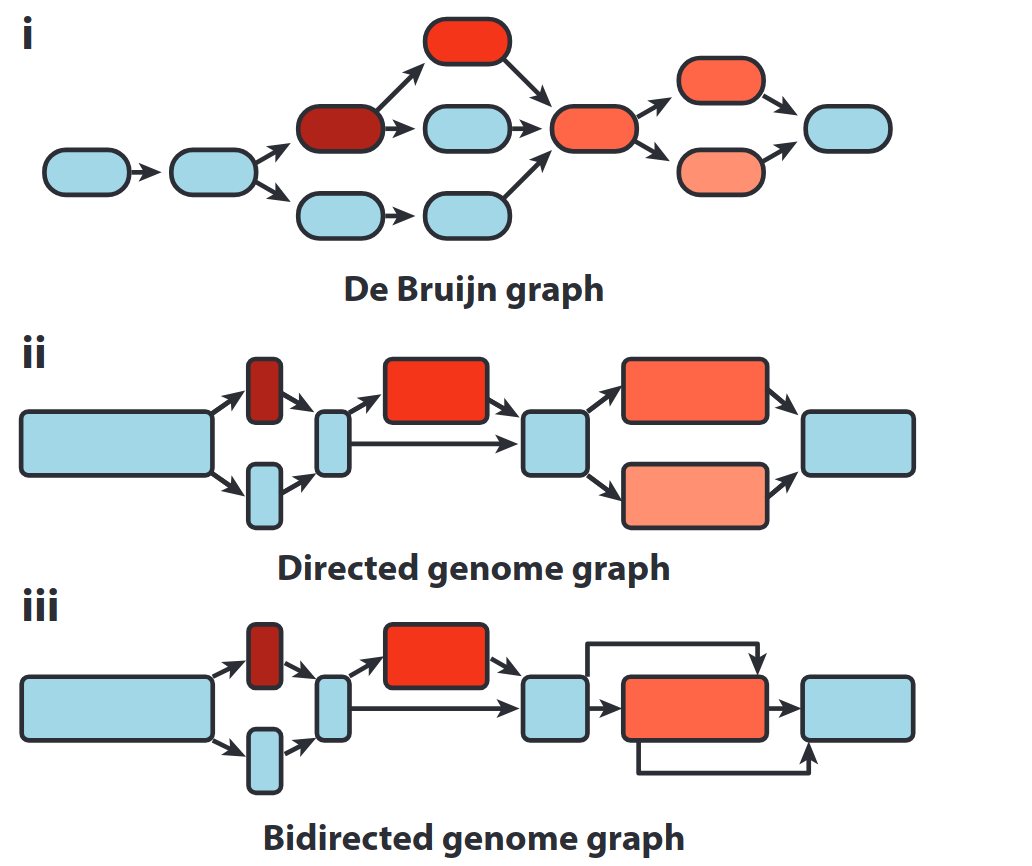
\includegraphics[width=.75\linewidth]{figures/background/graph_types.png}
	\caption[Graph pangenome models.]{The three main kind of graphs used to represent pangenomes. Figure from~\cite{eizenga}}
	\label{fig:graph_types.png}
\end{figure}
The choice of a particular model depends largely on the intended application, as there is no one-size-fits-all solution due to trade-offs between different desirable features. For instance, a model that facilitates effective visualization may not be suitable for handling large collections of genomes. Similarly, models that support the addition of new genomes without requiring complete recomputation—often referred to as dynamic updates—may not be the most efficient in terms of compression.\\
In the context of genomic variations represented in graphs, "bubbles" depict alternative paths between a source node and an end node. Different types of variations lead to distinct bubble structures, and different models generate bubbles with varying patterns. Examples of such bubbles for de Bruijn graphs and genome graphs are shown in Figures \ref{fig:vg_example} and \ref{fig:dbg_ex}.\\
Below, I introduce the two most widely used models for constructing pangenome graphs: Variation Graphs and De Bruijn Graphs.

\subsection{Variation Graphs}
Variation graphs are an enhancement of bidirected genome graphs with paths. Paths correspond to walks in the graph that visit nodes in an assigned orientation to reproduce sequences provided as input, as shown in figure~\ref{fig:vg_example}. It therefore consists of a bidirected genome graph constructed from the sequences in the input genomes plus a list of paths that spell such sequences inside the graph.
\begin{figure}[h!]
	\centering
	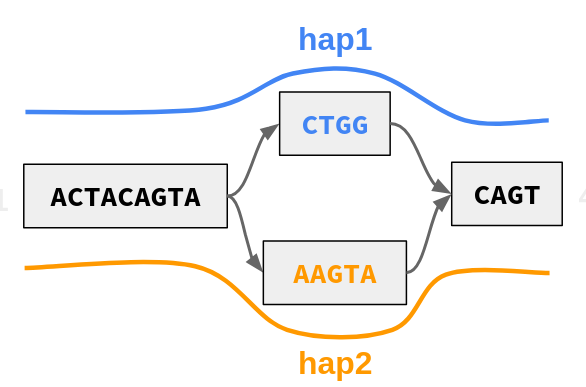
\includegraphics[width=.65\linewidth]{figures/background/vg.png}
	\caption[The Variation Graph model.]{An example of variation graph, in which haplotype1 spells the sequence \emph{ACTACAGTACTGGCAGT}, while haplotype 2 spells the sequence \emph{ACTACAGTAAAGTACAGT}~\cite{garrison_pangenome}.}
	\label{fig:vg_example}
\end{figure}
This data structure has been first proposed to represent textual variations. As shown in figure~\ref{fig:campagna_romana}, the variation graphs represent the conservation and variation in a system: it is therefore a very good model to represent the direct relationships between a group of genomes.
\begin{figure}[h!]
	\centering
	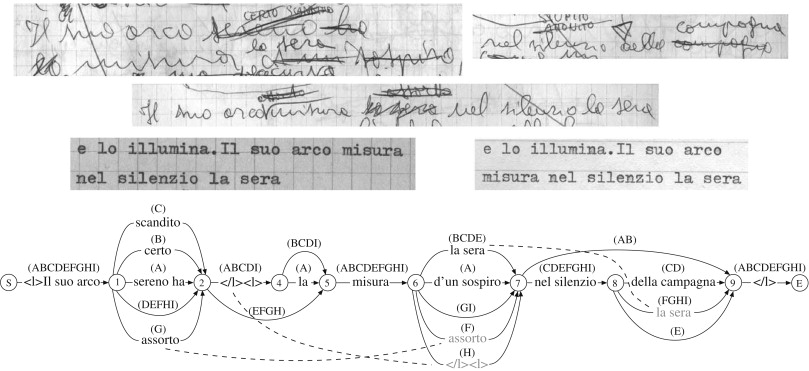
\includegraphics[width=.95\linewidth]{figures/background/variant_graph.jpg}
	\caption[The Variation Graph origin.]{Instead of having to preform all the pairwise comparisons of the nine version of Valerio Magrelli's "Campagna Romana" poem from 1981, the variation graph structure describes the differences between them. It also removes the high redundancy in the versions of the poem~\cite{variant_graph,garrison_pangenome}.}
	\label{fig:campagna_romana}
\end{figure}
Variation graphs of genomes can now be constructed thanks to the advent of TGS and complete high quality assembly pipelines. As already discussed, genomes are full of repeats, making assembly is hard, especially if the only information available is reads shorter than the repeat sequences, as with NGS.\\
Variation graphs can be generated in a direct, all-v-all unbiased way or in a iterative, reference driven manner.
%The pros of using a variation graph are:
%\begin{itemize}
%	\item variation is intuitive when visualizing the graph
%\end{itemize}



\subsection{De Bruijn Graphs}
\label{sec:dbg_intro}
Similar to variation graphs,  \dbgs were not originally developed for pangenomics. They are a well-known data structure that has been widely used in genome assembly, particularly in the context of Next Generation Sequencing.
A \dbg represents a collection of input sequences as a set of \kmers. By storing each unique \kmer only once, the structure reduces redundancy in the input data. In the graph, nodes are labeled with \kmers, and directed edges between nodes represent an overlap of $k-1$ bases between the two \kmers. \dbgs are also bidirected, as each \kmer includes its reverse complement; the version present in the node label is usually the canonical one. Bidirected edges thus encode the strand orientation of both the starting and ending \kmers.

\begin{figure}[h!]
	\centering
	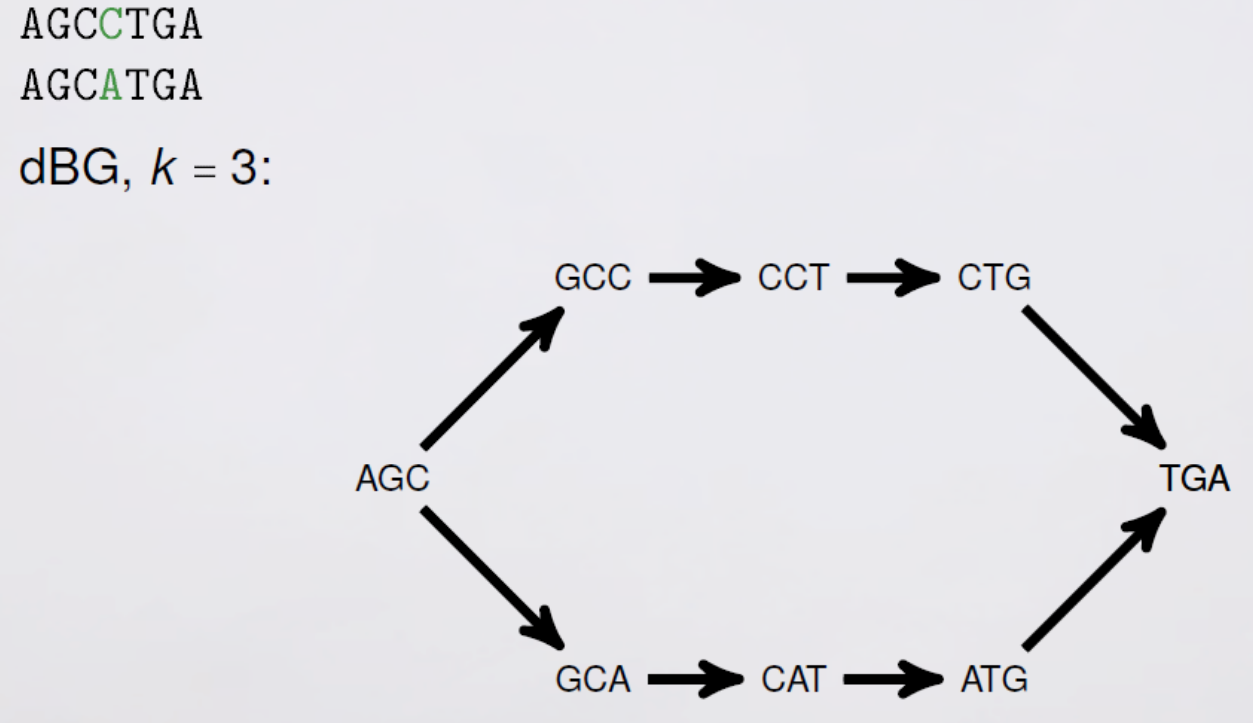
\includegraphics[width=.95\linewidth]{figures/background/dbg.png}
	\caption[Example of \dbg.]{Example of \dbg for $k=3$ with a bubble representing a SNP. Image made by Rayan Chikhi.}
	\label{fig:dbg_ex}
\end{figure}
The choice of $k$ depends on multiple factors and in fact is a trade-off between: 
\begin{itemize}
	\item[Specificity] The larger the $k$, the sparser is the set of \kmers of the \dbg in the space. While smaller $k$ (21-31) is more general and suitable for most applications, larger values of $k$ (61-100) provide greater specificity. The \kmers in genomes are not random and follow a skewed heavy-tail distribution~\cite{chor2009genomic}. Using larger $k$ value reduces the probability that two genomes share the same \kmer by chance.
	\item[Variation resolution]While variation is always encoded in the \dbg, using larger values of $k$ results in a sparser graph, where there are fewer nodes representing \kmers that occur multiple times in the genome. This implies that, when visualizing a specific region of the graph, it becomes easier to detect local variations without being confounded by nodes and edges coming from other parts of the genome that share the same \kmers as the region of interest.
	\item[Space] As shown in in table~\ref{tab-kmers}, larger value of $k$ produces more redundancy and a greater number of basepairs with the same input sequences. If the collection to study is large, smaller $k$ can provide beneficial features for disk storage or computational resources needed when using it.
\end{itemize}
\subsubsection{Colored and Compacted De Bruijn Graphs}
In order to produce a more compact and informative representation, in pangenomics it is used a particular version of the \dbg, called \ccdbg: colored compacted \dbg. The main characteristics of this data structure are:
\begin{itemize}
	\item Paths that do not contain any branches or bubbles are compacted into a single node. Given a chain of nodes in the graph, if the internal nodes have an in-degree of 1 and an out-degree of 1, the starting node has an out-degree of 1, and the final node has an in-degree of 1, the entire chain can be compacted into a single node. The resulting label is the extension of the first \kmer with the last nucleotide of the labels of the subsequent nodes. These compacted labels are no longer of length k and are thus not \kmers; they are referred to as unitigs, providing a more succinct representation of the \kmers in the de Bruijn graph, as shown in Figure~\ref{fig:ccdbg}.
	\item The genome of origin for each \kmer is recorded, and this information is referred to as its color, indicating which genomes the \kmer is present in. The color of each \kmer in the colored compacted de Bruijn graph is stored in a highly compressed format to minimize space usage. This color encoding enables more advanced analyses by allowing us to not only examine the presence or absence of a \kmer in the de Bruijn graph, but also to determine in which genomes the \kmer was observed.
\end{itemize}
While \kmer compaction into unitigs can be performed as a post-processing step starting from a de Bruijn graph, many modern methods compute unitigs directly, bypassing the need for constructing the full \dbg.\\
The term color can be somewhat confusing, as it is used in two distinct contexts: it may either refer to the dataset of origin for a \kmer, or it can represent any combination of datasets in which a \kmer is observed (commonly referred to as color sets)~\cite{marchet_kmersets}. The color set model is the most widely used, as it assigns an integer identifier to every unique combination of datasets in which a \kmer is found, instead of storing the precise dataset affiliations for each \kmer. This approach greatly reduces space usage, as illustrated in Figure~\ref{fig:ccdbg}. 
\begin{figure}[h!]
	\centering
	\begin{subfigure}[b]{0.95\textwidth}
		\centering
		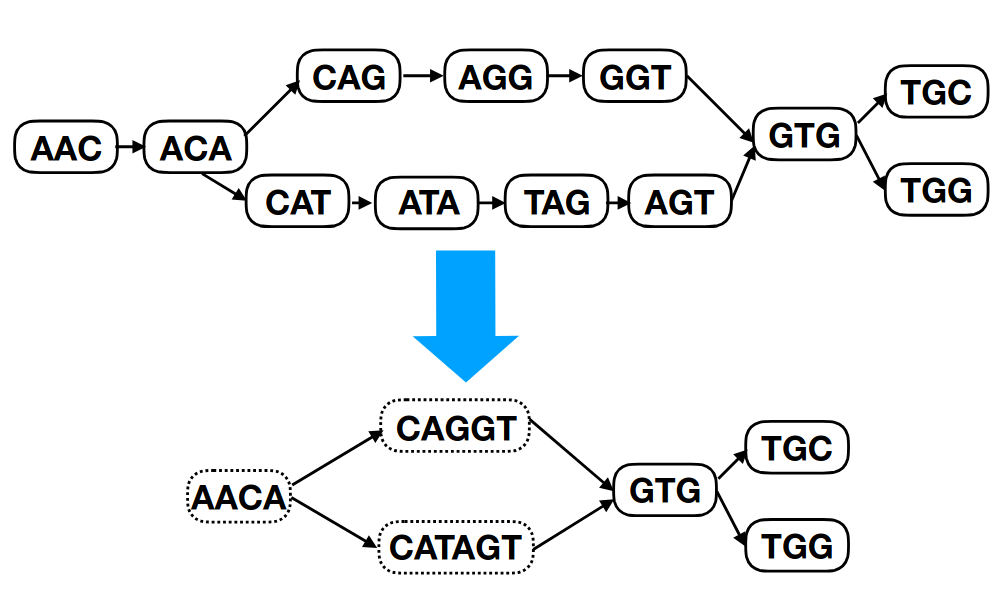
\includegraphics[width=.75\linewidth]{figures/background/compacting.png}
		\caption[Compacting a \dbg.]{Compacting a \dbg from the two sequences \texttt{AACAGGTGC} and \texttt{AACATAGTGG} into a \cdbg reduces paths of nodes with in-degree and out-degree of 1 into a single node. Figure from~\cite{embedding_dbg}}
	\end{subfigure}%
	\\
	\begin{subfigure}[b]{0.95\textwidth}
		\centering
		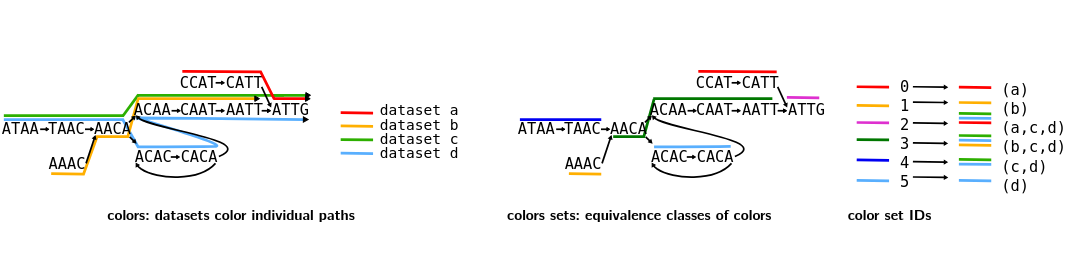
\includegraphics[width=0.95\textwidth]{figures/background/colors_dbg.png}
		\caption[The colors in a \ccdbg.]{The two kind of colors that can be used on \ccdbg: colors and color sets.} 
	\end{subfigure}
	\caption[Compaction and colors in a \ccdbg.]{Compaction and colors: the two main characteristic of a \ccdbg compared to a \dbg. Figure from~\cite{marchet_kmersets}}
	\label{fig:ccdbg}
\end{figure}
\section{Outline}
In the work presented below, we investigate the graphical pangenome representation on the features presented in the sections above. We focused mainly on the construction of such models, their underlying data structures and the downstream applications they enable.\\
The contributions presented in this manuscript are the following:
\begin{enumerate}
	\item \textbf{An analysis of pangenome construction methods and their applications}. Even if the variation graph model has been devised around 15 years ago, its application for pangenomics is very recent. \dbgs are instead a known model that has been extensively used for genome assembly and their application to pangenomics is relatively straightforward. We used all the state-of-the-art tools to produce a pangenome graph based on these two representations using a large collection of complete human genomes and tested computational resources, variation representation and applications.
	\item  \textbf{A novel construction of pathogenic yeast strains to discover chromosomal translocations.} Pangenome graphs can be used to investigate complex structural variations in genomes. In this case we sequenced, assembled and analyzed a group of 11 samples. We modified a variation graph construction pipeline to detect cross-chromosome events and discussed differences in the final representation.
	\item \textbf{A unitig matrix construction pipeline for presence/absence or counts.} We proposed a small pipeline, based on already published tools and a novel method, \kmat, a pipeline to build unitig matrices with abundances from a set of genomes via \kmer matrix and to directly generate a presence absence unitig matrix using \ccdbgs. 
	\item  \textbf{A novel super\kmers enumeration and sorting method.} We propose a novel way to encode and store super\kmers that preserves locality for the ones sharing the same minimizer to improve sequence queries. We also propose a tool to enumerate and sort super\kmers from a set of sequences using this model.
\end{enumerate}

The next chapters present this work and discuss the possible directions for future work based on it.

\printbibliography